%%%%%%%%%%%%%%%%%%%%%%%%%%%%%%%%%%%%%%

\documentclass[12pt]{article}
%\documentstyle[12pt,psfig,epsf]{article}

\hoffset=-15mm \voffset=-25mm \textwidth=165mm \textheight=245mm
\usepackage{graphicx}
\usepackage{amsmath}
\usepackage{amssymb}
%\usepackage{bigcircle}
\usepackage{wrapfig}
\usepackage{indentfirst}
\usepackage{color}
\usepackage{subfigure}

\begin{document}

\vskip 0.5cm \centerline{\bf\Large Low missing mass, single- and double diffraction }
\centerline{\bf\Large dissociation at the LHC}  \vskip 0.3cm
\vskip 1cm

\begin{abstract}
Low missing mass, single- and double diffraction dissociation are calculated for the LHC energies from a dual-Regge model dominated by a Pomeron Regge pole ex\-change. The model reproduces the rich resonance structure in the low missing mass, $M_X$ region. The diffractively excited states lie on the nucleon trajectory $N^*$, appended by the isolated Roper resonance. Detailed predictions for the squared momentum transfer and missing mass dependence of the differential and integrated single- and double diffraction dissociation in the kinematical range of present and future LHC measurements are given.
\end{abstract}

\section{Introduction}
Measurements of single (SD), double (DD) and central (CD) diffraction dissociation are among the priorities of the LHC research program.
Fig.~\ref{fig:FeynmanDiagrams} shows the simplest configurations of Regge-pole diagrams for elastic scattering, single- and double diffraction dissociation, as well as for central diffraction dissociation (CD). In this paper we consider only SD and DD.
% %%%%%%%%%%%%% 1 %%%%%%%%%%%%%%%%%
% %%%%%%%%%%%%%%%%%%%%%%%%%%%%%%%%%

In the past, intensive studies of high-energy diffraction dissociation were performed at the Fermilab,
on fixed deuteron target, and at the ISR \cite{Goulianos}. Fig.~\ref{fig1}(a)
shows representative data of low-mass SD as measured at the Fermilab.
One can see a rich resonance structure there, typical of low missing masses, often ignored by extrapolating the whole region by a simple $1/M^2$ dependence.

When extrapolating (in energy), one should however bear in mind that, in the ISR region, secondary Reggeon contributions are still important (their relative contribution depends on momenta transfer considered), amounting to nearly $50\%$ in the forward direction. At the LHC, however, their contribution in the nearly forward direction in negligible, i.e. less than the relevant error bars in the measured total cross section \cite{JLL}.
 
 In most of the papers on the subject, SD is calculated from the triple Regge limit of an inclusive reaction. %, as shown in Fig.~\ref{fig:TripleReggeLimit}.
In that limit, the double differential cross section can be written as \cite{Collins, Goulianos}
\begin{equation}
\frac{d^2\sigma}{dtdM^2_x}=
\frac{G^{PP, P(t)}_{1 3, 2}}{16\pi^2s_0^2}\left(\frac{s}{s_0}\right)^{2(\alpha_P(t)-1)}\left(\frac{M^2}{s_0}\right)^{\alpha_P(0)-2\alpha_P(t)}.
\end{equation}

This approach has two shortcomings. The first is that it leaves outside the small-$M^2$ resonance region. The second one is connected to the fact that whatever the Pomeron, the (partial) SD cross section overshoots the total one, thus obviously conflicting with unitarity. Various ways of resolving this deficiency
are known from the literature, including the vanishing (decoupling) of the triple Pomeron coupling, but none of them can be considered as completely satisfactory one.


We instead follow the idea put forward in paper \cite{JL} and developed further in \cite{PR}, according to which the Reggeon (here, the Pomeron) is similar to the photon and that the Reggeon-nucleon interaction is similar to deep-inelastic photon-nucleon scattering (DIS), with the replacement $-Q^2=q^2\rightarrow t$ and $s=W^2\rightarrow M^2_x$. There is an obvious difference between the two: while the $C$ parity of the photon is negative, it is positive for the Pomeron. We believe that while the dynamics is essentially invariant under the change of $C$, the difference between the two being accounted for by the proper choice of the parameters. Furthermore, while Jaroszewicz and Landshoff \cite{JL}, in their Pomeron-nucleon DIS structure function (SF) (or $\P p$ total cross section) use the Regge asymptotic limit, we include also the low missing mass resonance behavior. 

It is evident that Regge factorization is essential in both approaches (triple Regge and the present one). It is feasible when Regge singularities are isolated poles. While the pre-LHC data require the inclusion of secondary Reggeons, at the LHC we are in the fortunate situation of a single Pomeron exchange (Pomeron dominance) in the $t$ channel in single and double diffraction (not necessarily so in central diffraction). Secondary Regge pole exchanges will appear however, in our  dual-Regge treatment of $\P p$ scattering (see below), not to be confused with the $t$ channel of $pp$.
This new situation makes diffraction at the LHC unique in the sense that for the first time Regge-factorization is directly applicable. We make full use of it.

The paper is organized as follows: Sec. \ref{sec:preLHC} contains a short overview on the pre-LHC measurements of (mainly) single and double diffraction dissociation and their theoretical interpretation. Sec. \ref{sec:Factor} presents simple factorization relations connecting DD with elastic and SD cross sections. Next, in Sec. \ref{sec:Model} we introduce the dual-Regge model \cite{PR}, the (non-linear) $N^*$ Regge trajectory, the Roper resonance and summarize the main formulae used in our calculations. Fits to the data (figures an tables), presented in Sec. \ref{sec:Results}, are preceded by a brief introduction to our fitting strategy.
Sec. \ref{sec:Conclusions} summarizes our conclusions.

\section{Pre-LHC measurements: CERN ISR and SPS, Fermilab. Generalities} \label{sec:preLHC}
Diffraction dissociation was predicted by theory (for a historical review and relevant references see \cite{Goulianos, Kaidalov, Zotov}) and was intensively studied prior to the LHC on fixed deuteron targets at the Fermilab by a very successful Soviet-US collaboration \cite{Akimov}  and subsequently at the ISR, SPS and RHIC colliders \cite{Goulianos, Tsarev}. 
Together with high energy experiments (such as UA4, UA5, E710, CDF) the enerty range  $\sqrt{s}<1800$ GeV, transversal momentum $|t|<2$ GeV$^2$, and missing mass from  $M^2_{th}=(m_p+m_{\pi})^2$ up to $\xi<0.05$ (or even $\xi<0.15$), where $\xi=M^2_X/s$, was covered.
%%%%%%%%%%%%% 2 %%%%%%%%%%%%%%%%%
%%%%%%%%%%%%%%%%%%%%%%%%%%%%%%%%%

The main results of these measurements and of their theoretical interpretation can be summarized as follows:

%##########################################################################
1. {\bf Energy dependence.} At energies below 30~GeV the integrated SD cross section rises with $s$ according to the standard prescription of the Regge-pole theory, however it slows down beyond.
This effect was expected due to the familiar problem related to the violation of unitarity, namely that at high energies, implying the triple Pomeron limit, the SD cross section overshoot the total cross section, $\sigma_\mathrm{SD}>\sigma_t(s).$ Various means were suggested \cite{triple} to remedy this deficiency, including decoupling (vanishing) of the triple
Pomeron vertex. Goulianos instead renormalizes the standard Pomeron flux to meet the data \cite{Goulianos1}. Such a ``renormalization'' produces a break near $\sqrt s$ slowing down the rise of $\sigma_\mathrm{SD}(s)$ in accord with the CDF data from the Tevatron, as shown in Fig.~\ref{fig1}.

An alternative approach intended to resolve this crises (violation of unitarity) is based on the use of double Pomeron pole ~\cite{JMPP}.

%%%%%%%%%%%%%%%%%%%%%%%%%%%%%%%%%%%%
2. {\bf $t-$ dependence.}
As expected, SD and DD are peaked in the forward direction, and the slope of the exponential peak of SD was found to be around $8\div12$~GeV$^{-2}$, varying with $s,\ t$ and $M^2$.
 
A diffraction minimum around $t\approx 1$~GeV$^2$, similar to that in elastic hadron scattering, is expected also in SD (and DD). There are indications \cite{dip} of such a structure in $pp\rightarrow p(n\pi^+)$ at rather small $|t|$, around $|t|\sim 0.2\div 0.3$~GeV$^2$ at $\sqrt s=53$~GeV, however its relation to the dip-bump structure in elastic scattering is still a matter of debate \cite{JLL}.

Diffraction is limited both in the missing mass $\xi\lesssim 0.05$ (coherence condition) and in $t$ (``soft'' collisions). There is a transition region in $t$ from ``soft'' to ``hard'' collisions, with a possible dip-bump structure between the two. To be sure, in our analysis we leave outside these interesting but controversial points, concentrating only on the ``first'' cone with exponential behavior at small $t<0.5$ GeV$^2$.

%###########################################################################
3. {\bf $M^2$ dependence.} 
First SD measurements, e.g. in the reaction $pp\rightarrow pX$ (or $pI\P\rightarrow X$), investigated low missing masses near the threshold region $M_{th}=(m_p+m_{\pi})$. In that region, resonance peaks were revealed, see Figs.~\ref{fig1}(a) . The origin and properties of theses peaks, still subject of debates. The main deficiency of the missing mass method, that was used, is the lack of any information on the decay properties of the produced particles. 
%The missing information was obtained in bubble chamber experiments and in spark chambers, used also in exclusive channels at the ISR Collider.

Apart from low missing masses, SD was found to persist also at high missing masses. Coherence contidions imposes,  an upper limit on the highest missing masses $M_x$ of SD,  $\xi=M^2_X/s\lesssim0.05$.

%%%%%%%%%%%%%%%%%%

In most of the papers on the subject, this resonance structure is ignored and replaced by a smooth function $\sim M^{-2}$ descring the region of larger missing masses. In Secs. \ref{sec:Model} and \ref{sec:Results} we question this point on the following reasons: a) The low-$M^2$, resonances introduce strong irregularities in the behavior of the resulting cross sections. LHC measurements, are able to probe the low-$M^2$ region, and will be sensitive to these structures. b) The large-$M$ behavior of the amplitude (cross sections) is another delicate point. Essentially, it is determined by the proton-Pomeron ($p\P$) total cross section, proportional to the $p\P$ structure function, discussed in details in Sec. \ref{sec:Model}.
By duality, the averaged contribution from resonances sums up to produce high missing mass Regge behavior $~(M^2)^{-n},$ where $n$ is related to the intercept of the exchanged Reggeon and may be close (but not necessarily equal) to the above-mentioned empirical value $\sim 1$.

In our calculations of the large-$M$ behavior (Secs. \ref{sec:Model} and \ref{sec:Results}) we shall refer also to the ISR-Tevatron-CDF data, remembering that for low energies ($\lesssim500$~GeV), non-leading Regge exchanges are also important \cite{JLL}.

\section{Simple (and approximate) factorization relations} \label{sec:Factor}
With the advent of the LHC, diffraction, elastic and inelastic scattering entered a new area, where it can be seen uncontaminated by non-diffraction
events. In terms of the Regge-pole theory this means, that there is a region, where the scattering amplitude is completely determined by Pomeron exchange, and in a
simple-pole approximation Regge factorization holds and it is of practical use! Remind that the Pomeron is not necessarily a simple pole:
perturbative QCD suggests that the Pomeron is made of an infinite number of poles (useless in practice), and the unitarity condition requires corrections
to the simple pole, whose calculation is far from unique. Instead, a simple Pomeron pole approximation \cite{DL} is efficient in describing
a variety of diffraction phenomena.
%
The D-L elastic scattering amplitude \cite{DL} is simply
\begin{equation}\label{DL}
A(s,t)=\xi(t)\beta^2(t)(s/s_0)^{\alpha_P(t)-1}+A_{Reg}(s,t),
\end{equation}
where $\xi(t)$ is the signature factor, and $\alpha(t)$ is the (linear) Pomeron trajectory. The signature factor can be
written as $\xi(t)=e^{-\frac{i\pi\alpha_{\!\P}(t)}{2}}$ (see \cite{PR}), however it is irrelevant here, since below we shall use only cross sections (squared modules of the amplitude), where it reduces to unity. The residue is chosen to be a simple exponent, $\beta(t)=e^{b_Pt}$.
``Minus one'' in the propagator term $(s/s_0)^{\alpha_{\!\P}(t)-1}$ of (\ref{DL}) correspond to normalization $\sigma_T(s)=Im A(s,t=0)$. The scale parameter $s_0$ is not fixed by the Regge-pole theory: it can be fitted do the data or fixed to a ``plausible'' value of a hadronic mass, or to the inverse ``string tension'' (inverse of the Pomeron slope), $s_0=1/\alpha'$. The second term $A_R(s,t)$ in Eq.~(\ref{DL}), corresponding to sub-leading Reggeons, has the same functional form as the first one (that of the Pomeron), just the values of the parameters differ.
We ignore this term for reason mentioned above.


Factorization of the Regge residue $\beta(t)$ and the ``propagator'' $(s/s_0)^{\alpha_P(t)-1}$ is a basic property of the theory. As mentioned, at the LHC for the first time
we have the opportunity to test directly Regge-factorization  in diffraction, since the scattering amplitude here is dominated by a simple Pomeron-pole exchange, identical in elastic and inelastic diffraction.
Simple factorization relations between elastic ($\frac{d\sigma_\mathrm{el}}{dt}$), single ($\frac{d\sigma_\mathrm{el}}{dt})$ and double ($\frac{d^3\sigma_\mathrm{DD}}{dtdM_1^2dM_2^2})$ DD are known from the literature \cite{Goulianos}.
Really, by writing the scattering amplitude as a product of the vertices, elastic $f$ and inelastic $F$, multiplied by the (universal) propagator (Pomeron exchange), we obtain $f^2s^{\alpha}$, $fFs^{\alpha}$, $F^2s^{\alpha}$ for elastic scattering, SD and DD, respectively, and one gets
\begin{equation}\label{factor1}
\frac{d^3\sigma_\mathrm{DD}}{dtdM_1^2dM_2^2}=\frac{d^2\sigma_\mathrm{SD1}}{dtdM_1^2}\frac{d^2\sigma_\mathrm{SD2}}{dtdM_2^2}/\frac{d\sigma_\mathrm{el}}{dt}.
\end{equation}

%####### sec ######
\section{Model for single and double diffraction dissociation}\label{sec:Model}
The model relies on the following premises:

1.  {\bf Regge factorization} is feasible since, as stressed repeatedly, at the LHC energies in the region of $|t|<1$~GeV$^2$, which is typical for diffraction, the contribution from secondary Reggeons is negligible, and, for a single Pomeron term, factorization (\ref{factor1}) is exact. Due to factorization, the relevant expressions for the cross sections (elastic, SD, DD) have simple forms (\ref{elastic}), (\ref{SD}), (\ref{DD}). Such relations are known from the literature, see eg. \cite{Goulianos, Chew:1974zy,Chew:1974vu} and references therein.

2. {\bf The inelastic $p\P X$ vertex} receives special care.

Having justified and accepted the factorized form of the scattering amplitude,
the main object of our study is now the inelastic proton-Pomeron vertex or transition amplitude.
As argued in Refs. \cite{JL,PR}, it can be treated as the proton structure function (SF), probed by the Pomeron, and proportional to the

Pomeron-proton total cross section, $\sigma_T^{\P p}(M^2_x, t),$ with the norm $\sigma_T^{\P p}(M^2_x, t)=\Im\, A(M^2,t),$
in analogy with the proton SF probed by a photon (in $ep$ scattering e.g. at HERA or JLab).
\begin{equation}
 %\begin{array}{ll}
 \label{SF}
   \nu W_2(M_x^2,t)=F_2(x,t)\sim \frac{(-t)(1-x)^2}{(M_x^2-m_p^2)(1+4m_p^2x^2/(-t))^{3/2}}\Im A(M^2,t),
% \end{array}
\end{equation}
where $\nu=\frac{M_x^2-m_p^2-t}{2m_p}$, and $x=\frac{-t}{2m_p\nu}$ is the Bjorken variable\footnote{This relation is valid in the large-$|t|$ and the large-$M_x^2$ Bjorken limit. Its validity and possible consequences in the low-$|t|$ region is disputable. In the present paper we avoid the low-$|t|$ approximation of Eq.~(\ref{SF}).}.


The only difference is that the Pomeron's (positive) $C$ parity is opposite to the photon's parity. This difference is evident in the values of the parameters but is unlikely to affect the functional form of the SF itself, for which we choose its high-$M_x^2$ (low Bjorken $x$) behavior. Notice that the total energy in this subprocess, the analogy of $s=W^2$ in DIS, here is $M^2_x$ and $t$ here replaces $q^2=-Q^2$ of DIS.
%Notice that gauge invariance requires that the SF vanishes towards $Q^2\rightarrow 0$ (here $t$), resulting in the dramatic vanishing of the SD and DD differential cross section towards $t=0$.  How fast does the SF (and relevant cross sections) recover from $t=0$ a priori is not known.

Furthermore, according to the ideas of two-component duality, see e.g. \cite{JPsi}, the cross sections of any process, including that of $p\P\rightarrow X,$ is a sum of a non-diffraction component, in which resonances sum up in high-energy (here: the mass $M^2_x$ plays the role of energy $s$) Regge exchanges and the smooth background (below the resonances), dual to the Pomeron exchange (see Fig.~\ref{fig:Regge-dual}). The dual properties of diffraction dissociation can be quantified also by finite mass sum rules, see \cite{Goulianos}. In short: the high-mass behavior of the $p\P\rightarrow X$ cross section is a sum of a decreasing term going like $\sim \frac{1}{M^m}$, $m\approx 2$ and a ``Pomeron exchange'' increasing slowly with mass. 

3. {\bf The background} is a delicate issue. In the reactions (SD, DD) under consideration there are two sources of the background. The first is that related to the $t$ channel exchange in Fig.~\ref{fig:FeynmanDiagrams} and it can be accounted for by rescaling the parameter $s_0$ in the denominator of the Pomeron propagator. In any case, at high energies, those of the LHC, this background is included automatically in the Pomeron. The second component of background comes from the subprocesses $p\P\rightarrow X$. Its high-mass behavior is not known experimentally and it can be only conjecture on the bases of the known energy dependence of the typical meson-baryon processes appended by the ideas of duality. The conclusion is that the $\P p$ total cross section at high energies (here: missing masses $M$) has two components:
 a decreasing one, dual to direct-channel resonances and going as $\sigma_\mathrm{tot}^{\P p}\sim \sum_R(s')^{\alpha_R(0)-1}= \sum_R\left(M^2\right)^{\alpha_R(0)-1},$ where $R$ are non-leading Reggeons, and a slowly rising Pomeron term producing $\sim M^{2\cdot0.08}$ \cite{DL}.
%####### SubSec ######
\subsection{Duality} \label{subsec:Duality}
Any meson-baryon total cross section (or scattering amplitude) is a sum of two contributions: diffractive and non-diffractive. By the concept of two-component duality \cite{H_R},
the diffractive component is a smooth background at low energies (here: missing masses) and dual to a Pomeron $t$-channel exchange at high energies, while the non-diffractive
component contains direct channel resonances, and is dual to high-energy $t-$ channel (sub-leading) Reggeon exchanges, as shown in Fig.~\ref{fig:Regge-dual}.
%%%%%%%%%%%%% 3 %%%%%%%%%%%%%%%%%
%%%%%%%%%%%%%%%%%%%%%%%%%%%%%%%%%

According to our present knowledge about two-body hadronic reactions, two distinct classes of reaction mechanisms exist.

The first one includes the formation of resonances in the $s-$channel
and the exchange of particles, resonances, or Regge
trajectories in the $t-$channel. The low-energy resonance
behavior and the high-energy Regge asymptotics are related by
duality, that, at Born level, or,
alternatively, for tree diagrams, mathematically can be formalized
in the Veneziano model, which is a combination of Euler
Beta-functions \cite{Veneziano}.

The second class of mechanisms does not exhibit resonances at low
energies and its high-energy behavior is governed by the exchange
of a vacuum Regge trajectory, the Pomeron, with an intercept equal
to or slightly greater than one. Harari and Rosner \cite{H_R}
hypothesized that the low-energy non-resonating background is dual
to the high-energy Pomeron exchange, or diffraction. In other
words, the low-energy background should extrapolate to high-energy
diffraction in the same way as the sum of narrow resonances sum up
to produce Regge behaviour. However, contrary to the case of
narrow resonances, the Veneziano amplitude, by construction,
cannot be applied to (infinitely) broad resonances. This becomes
possible in a generalization of narrow resonance dual models
called dual amplitudes with Mandelstam analyticity (DAMA),
allowing for (infinitely) broad resonances, see \cite{DAMA} and references therein, or
the background.


In the resonance region, roughly $1\lesssim M\lesssim 4$~GeV, the non-diffractive component of the amplitude is adequately described by a ``reggeized Breit-Wigner'' term  Eq.~(\ref{total}), following from the low-energy decomposition of a dual amplitude, with a direct-channel meson-baryon (Pomeron-proton, in our case) trajectory (Fig.~\ref{fig:n1}), with relevant nucleon resonances lying on it, appended by the Roper resonance (see Eq.~(\ref{Roper_eq})).

%  \begin{table}
%  \centering
%  \caption{Two-component duality}\label{tab1}
%  \begin{tabular}{|l|l|l|}
%  %\begin{tabular}{\columnwidth}{@{\extracolsep{\fill}}|l|l|l|@{}}
%    \hline
%    $\Im A(ab\rightarrow cd)$& $R$& Pomeron \\
%    \hline
%    $s-$channel & $\sum A_{Res}$  & Non-resonant background \\
%    $t-$channel & $\sum A_{Regge}$ & Pomeron\\
%                &                  &$(I=S=B=0;\ C=+1)$ \\
%    High energy &$s^{\alpha-1},\ \alpha<1$&$s^{\alpha-1},\ \alpha\geq 1$ \\
%     dependence&&\\
%    \hline
%  \end{tabular}
%  \end{table}
 
By duality, a proper sum of direct channel resonances produces smooth Regge behavior, and, to avoid ``double counting'', one should not add the two. Actually, this is true only for an infinite number of resonance poles. For technical reasons, we include only a finite number of resonance poles, moreover, apart from the ``regular'' contribution of the nucleon resonances, lying on the $N^*$ trajectory, the Roper resonance is also included (see Sec.~4.3). The spectroscopic status of this resonance is disputable. It has no place on the known baryonic trajectories, but its height exceeds that of the neighboring, $N^*(1680)$. In view of the ``truncated'' series of resonance poles, we do not expect that it will reproduce correctly the high-energy Regge behavior, therefore we add it to the total cross section in the form of an ``effective'' Regge pole contribution (background).

The second, diffractive component, is essentially the contribution from a Pomeron pole exchange
%
{\footnotesize $\sigma^{\P p}_T\sim M^{2(\alpha(0)-1)}$}, with $\alpha(0)\approx 1.08$ \cite{DL},
and, as shown by Donnachie and Landshoff \cite{DL}, this term also contribute to the low-energy (here, missing mass) flat background (also its main contribution comes from the region of high missing mass).

To summarize this discussion, Regge-pole exchanges take place at two distinct parts of the diagrams shown in Fig.~\ref{fig:FeynmanDiagrams}: in the $t$ channel, where, at the LHC, only the Pomeron contributes, and in the inelastic form factor, where, depending of the value of the missing mass, both the Pomeron and Reggeons are equally important. At low missing masses, the direct-channel proton trajectory $N^*$, dominates, replaced by an effective Reggeon exchange at high masses, appended by a Pomeron. The Roper resonance (with its controversial status) in the direct channel stays apart. Although we concentrate on the low missing mass region, the behavior of the cross sections at high masses are important in the calculation of the cross sections integrated in $M^2$. We remind that we impose a limit on diffraction events to be about $\xi<0.05$ or $M<200$~GeV (as it used at some experiments).

%####### SubSec ######
\subsection{Resonances in the $\P p$ system; the $N^*$ trajectory}\label{Sec:trajectory}
The $\P p$ total cross section at low missing masses is dominated by nucleon resonances. In the dual-Regge approach \cite{PR}, the relevant cross section is a ``Breit-Wigner'' sum Eq.~(\ref{total}), in which the direct-channel trajectory is that of $N^*$. An explicit model of the nonlinear $N^*$ trajectory was elaborated in paper \cite{Paccanoni} and used in \cite{PR}.
\begin{eqnarray}\label{total}
\sigma^{\P p}_T(M_x^2,t)=&\Im\, A(M_x^2,t)=
    \,\Im\left(\sum_{n=0,1,...}\frac{a f(t)^{2(n+1)}}{2n+0.5-\alpha_{N^*}(M_x^2)}\right).\nonumber 
\end{eqnarray}

The Pomeron-proton channel, $\P p\rightarrow M_X^2$  couples to the
proton trajectory (also called $N^{*}$ trajectory), with the $I(J^P)$ resonances: $1/2(5/2^+)$,
$F_{15}$, $m=1680$~MeV, $\Gamma=130$~MeV; $1/2(9/2^+)$ $H_{19}$ 
$m=2200$~MeV, $\Gamma=400$~MeV; and $1/2(13/2^+)$ $K_{1,13}$,
$m=2700$~MeV, $\Gamma=350$~MeV.
%%%%%%%%%%%%% 4 %%%%%%%%%%%%%%%%%
%%%%%%%%%%%%%%%%%%%%%%%%%%%%%%%%%
The status of the first two is
firmly established \cite{particles}, while the third one,
$N^*(2700),$ is less certain, with its width varying between
$350\pm 50$ and $900\pm 150$~MeV . Still, with the
stable proton included, we have a fairly rich trajectory,
$\alpha(M^2)$, whose real part is shown in Fig.~\ref{fig:n1}.


Despite the seemingly linear form of the trajectory, it is not
that: the trajectory must contain an imaginary part corresponding
to the finite widths of the resonances on it. The non-trivial
problem of combining the nearly linear and real function with its
imaginary part was solved in Ref.~\cite{Paccanoni} by means of
dispersion relations.

We use  the explicit form of the trajectory derived in Ref.~
\cite{Paccanoni}, ensuring  correct behaviour of both its real and
imaginary parts. The imaginary part of the trajectory can be
written in the following way:
\begin{equation}
\Im\, \alpha(s)=s^{\delta} \sum_n c_n
\left(\frac{s-s_n}{s}\right)^{\lambda_n} \cdot \theta(s-s_n)\,,
\label{b2}
\end{equation}
where $\lambda_n=\Re\ \alpha(s_n)$. Eq.~~(\ref{b2}) has the
correct threshold behaviour, while analyticity requires that
$\delta <1$. The boundedness of $\alpha(s)$ for $s \to \infty$
follows from the condition that the amplitude, in the Regge form,
should have no essential singularity at infinity in the cut plane.

The real part of the proton trajectory is given by
\begin{equation}
\Re\,\alpha(s)=\alpha(0)+\frac{s}{\pi}\sum_n c_n {A}_n(s)~, \label{b3}
\end{equation}
where
\begin{eqnarray}
 &{A}_n(s)=
\frac{\Gamma(1-\delta)\Gamma(\lambda_n+1)}{\Gamma(\lambda_n-\delta+2)
s_n^{1-\delta}}{}_2F_1\left(1,1-\delta;\lambda_n-\delta+2;\frac{s}{s_n}\right)\theta(s_n-s)\\ \nonumber
&+\left\{ \pi s^{\delta-1}\left(\frac{s-s_n}{s}\right)^{\lambda_n} \cot[\pi(1-\delta)]- \right. 
\left.\frac{\Gamma(-\delta)\Gamma(\lambda_n+1)s_n^{\delta}}{s\Gamma(\lambda_n-\delta+1)
}{}_2F_1\left(\delta-\lambda_n,1;\delta+1;\frac{s_n}{s}\right)
\vphantom{\left( \frac{s-s_n}{s}\right)^{\lambda_n}} \right \}
\theta(s-s_n),
\end{eqnarray}
where  $n=1,2,x$, $s_1=(m_{\pi}+m_N)^2=1.16$~GeV$^2$, $s_2$ = 2.44~GeV$^2$ and
$s_x$ = 11.7~GeV$^2$, and 
$\alpha(0)=-0.41$, $\delta = -0.46 \pm 0.07$, $c_1=0.51\pm 0.08$, $c_2=4.0\pm 0.8$ and $c_x=(4.6 \pm 1.7)\cdot
10^{3}$ (for details see \cite{JMPx}). 
Taking the central values of these parameters for $\lambda_n=\Re\, \alpha(s_n)$,  we obtain
the following values $\lambda_1=0.846$, $\lambda_2=2.082$, $\lambda_x=11.177$.

The elastic contribution, is separated from SD and DD by a gap extending from the proton mass $m_p$ to the first threshold, at $m_p+m_{\pi},$
and it should be treated separately.

 Thus, we obtain:
\begin{equation}\label{ImA_fin}
    \sigma_{t}^\mathrm{res}=\Im\, A(M_X^2,t)=     a\sum\limits_{n=1,3}[f(t)]^{2(n+1)}
    \frac{\Im\alpha(M^2_X)}{(2n+0.5-Re\, \alpha(M_X^2))^2+(\Im\, \alpha(M_X^2))^2}\,.%\nonumber
\end{equation}

\subsection{The Roper resonance \label{Roper}}
Apart from the well established protonic trajectory
with a sequence of four particles, there is a prominent single resonance
$I=1/2,\ \  J=1/2^+$ with mass $1440$~MeV, known as the Roper
resonance \cite{particles}. It is wide, the width being nearly one
fourth of its mass, its spectroscopic status being disputable.
There is no room for the Roper resonance on the proton trajectory
of Sec.~4.2, although it could still be a member of protons
daughter trajectory. Waiting for a future better understanding of Roper's status, here we
present the contribution to SD cross section of a single Roper
resonance, calculated from a simple
Breit-Wigner formula:
\begin{equation}\label{Roper_eq}
 \sigma_{t}^\mathrm{Roper}=\Im\, A_\mathrm{Roper}(M_x^2,t)=
c\frac{f^2(t) M_\mathrm{Roper} \Gamma_\mathrm{Roper}/2 }{(M^2_x - M^2_\mathrm{Roper})^2 + (\Gamma_\mathrm{Roper}/2)^2},
\end{equation}
where $M_\mathrm{Roper} = 1440$~MeV, $\Gamma_\mathrm{Roper} = 325$~MeV,  and $c$ is another normalization parameter.

%####################################################################
\subsection{Compilation of the basic formulae}
This subsection contains a compilation of the main formulae used in the calculations and fits to the data.

The elastic cross section is:
  \begin{equation}\label{elastic}\frac{d\sigma_\mathrm{el}}{dt}=A_\mathrm{el}{F_p}^4(t)\left(\frac{s}{s_0}\right)^{2(\alpha(t)-1)}.\end{equation}
The single diffraction (SD) dissociation cross section is:
  \begin{equation}\label{SD}2\cdot\frac{d^2\sigma_\mathrm{SD}}{dtdM_x^2}={F_p}^2(t){F_\mathrm{inel}}^2(t,M_x^2) \left(\frac{s}{M_x^2}\right)^{2(\alpha(t)-1)}.\end{equation}
The double diffraction dissociation (DD) cross section:
\begin{eqnarray}\label{DD}
   \frac{d^3\sigma_\mathrm{DD}}{dtdM_1^2dM_2^2}%\hspace{5cm}\\
    =N_\mathrm{DD}{F_\mathrm{inel}}^2(t,M_1^2){F_\mathrm{inel}}^2(t,M_2^2)
   \left(\frac{ss_0}{M_1^2M_2^2}\right)^{2(\alpha(t)-1)}, % \nonumber
\end{eqnarray}
with the norm $N_\mathrm{DD}=\frac{1}{4A_\mathrm{el}},$
where 
  \begin{equation}\label{eq:inelVertex}
   {F_\mathrm{inel}}^2(t,M_x^2)=A_\mathrm{res}\frac{1}{M_x^4}\sigma_T^{\P p}(M_x^2,t)+C_\mathrm{bg}\sigma_{Bg}(M_x^2,t),
  \end{equation}
and, for simplicity, the factor coming from $\frac{W_2(M_x^2,t)}{2m_p}$ (see Eq.~(\ref{SF})), proportional to the inelastic vertex, has been replased by $\frac{1}{M_x^4}$ (see also Eqs.~(7), (16) from \cite{PR}).  

The Pomeron-proton total cross section is the sum of $N^*$ resonances (the $t$ dependent term $[f_\mathrm{res}(t)]^{2(n+1)}$ from Eq.~(\ref{ImA_fin}) has been simplified to $f^4(t)$) and the Roper resonance Eq.~(\ref{Roper_eq}), with a relevant normalization factor $R$:
  \begin{eqnarray}
   \label{eq:sigma_tot}
    &\sigma_T^{\P p}(M_x^2,t)=&
    R\frac{[f_\mathrm{res}(t)]^{2} \cdot M_\mathrm{Roper}\left(\frac{\Gamma_\mathrm{Roper}}{2}\right)}
    {{\left(M_x^2-M_\mathrm{Roper}^2\right)}^2+{\left(\frac{\Gamma_\mathrm{Roper}}{2}\right)}^2}\\%\hspace{1.5cm}%\\
    %\;
    &&+[f_\mathrm{res}(t)]^{4}\sum_{n=1,3} \frac{\Im\,\alpha(M^2_x)}{(2n+0.5-\Re\, \alpha(M_x^2))^2+(\Im\,\alpha(M^2_x))^2},\nonumber
  \end{eqnarray}
and the background corresponding to non-resonance contributions\footnote{$[M_x]=[m_p]=[m_{\pi}]=[$GeV$]$.}:
  \begin{equation}\label{eq:sigma_bg}
   \sigma_{Bg}(M_x^2,t)=\frac{f_\mathrm{bg}(t)}{\frac{1}{{\left(M_x^2-(m_p+m_{\pi})^2\right)}^\varsigma}+(M_x^2)^{\eta}},
  \end{equation}
  

 The Pomeron trajectory (\cite{JLL}), the  $t-$dependente elastic and inelastic form factors  was set to $\alpha(t)=1.075+0.34t,$ $F_p(t)=e^{b_\mathrm{el}t},$ $f_\mathrm{res}(t)=e^{b_\mathrm{res}t},$ $f_\mathrm{bg}(t)=e^{b_\mathrm{bg}t}.$

 The slope of the cone is defined as\footnote{$\left[\frac{d\sigma}{dt}\right]=mb\cdot$GeV$^{-2}$.}:
  \begin{equation}\label{eq:B}
    B=\frac{d}{dt}\ln\frac{d\sigma}{dt},
  \end{equation}
where $\frac{d\sigma}{dt}$ stands for $\frac{d\sigma_\mathrm{el}}{dt},$  $\frac{d\sigma_\mathrm{SD}}{dt},$ or $\frac{d\sigma_\mathrm{DD}}{dt}$,  defined by Eq.~(\ref{elastic}), (\ref{SD}) and  (\ref{DD}), respectively.

  

  Partialy integrated cross sections for SD are calculated as:
  \begin{equation}\label{eq:dcsdt_SD}
    \frac{d\sigma_\mathrm{SD}}{dt}=\int_{M^2_1}^{M^2_2}\frac{d^2\sigma_\mathrm{SD}}{dtdM_x^2}dM_x^2,
  \end{equation}
  and for the case of DD:
  \begin{equation}\label{eq:dcsdt_DD}
    \frac{d\sigma_\mathrm{DD}}{dt}= \int\int_{f(M^2_{x_1},M^2_{x_2})}\frac{d^3\sigma_\mathrm{SD}}{ dtdM_{x_1}^2 dM_{x_2}^2 }dM_{x_1}^2dM_{x_2}^2.
  \end{equation}

  We also calculate the fully integrated cross sections:
  \begin{equation}
  \sigma_\mathrm{SD}=\int_{0}^{1}dt\int_{M^2_{th}}^{0.05s}dM_{x}^2 \frac{d^2\sigma_\mathrm{SD}}{dtdM_{x}^2},
  \end{equation}
  \begin{equation}
   \sigma_\mathrm{DD}=\int_{0}^{1}dt\int\int_{\Delta\eta>3}dM_{x_1}^2dM_{x_2}^2 \frac{d^3\sigma_\mathrm{DD}}{dtdM_{x_1}^2dM_{x_2}^2},
  \end{equation}
  %where $\Delta\eta=\ln\left(\frac{ss_0}{M_1^2M_2^2}\right)$
  and
  \begin{equation}
  \frac{d^2\sigma_\mathrm{DD}}{dM_{x_1}^2dM_{x_2}^2}= \int_{0}^{1}\frac{d^3\sigma_\mathrm{DD}}{dtdM_{x_1}^2dM_{x_2}^2}dt.
  \end{equation}

%####################################################################
%####################################################################
\section{Fitting procedure and results}\label{sec:Results}
The model contains 12 parameters. The fitting strategy consist of following parts.
%, a large part of which is fixed either by their standard values (e.g. those of Regge trajectories, except for the Pomeron slope, whose slope exceeds the ``standard'' value to meet the SD data) or are set close to the previous fits \cite{PR}.

\begin{itemize}
 \item In our strategy we  first adjust the model to ``standard candles'' of {\bf elastic $pp$ scattering} at high energies. We considered only the data corresponding to the first cone, described by a linear exponential, implying also a linear Pomeron trajectory.

 The elastic data and Regge theory fix the parameters  $s_0, \alpha(0)$, $\alpha'$, $A_\mathrm{el}$, $b_\mathrm{el}$.
 Theparameter $s_0$  is strongly correlated with the slope parameters $b_\mathrm{el}$, $b_\mathrm{res}$ and $b_bg$.
 As input data, the slope of diffraction cone ( see Table \ref{tab:cs.el}), and TOTEM elastic differential cross sections \cite{[T1].TOTEM, [T2].TOTEM} at $\sqrt{s}=7$~TeV were used.

% \textbf{The  data at larger $|t|$, with the dip-bump structure and subsequent flattening of the cross section, both in elastic scattering and in SD may indicate the onset of new physics and the transition to hard scattering, implying a non-exponential residue and/or a non-linear Pomeron trajectory, see Refs. \cite{JLL}, that goes beyond the present study.}

%############### tab 1 #######################
%#############################################

\item {\bf Single diffraction dissociation (SD)} is an important pillar in our fitting procedure.

In particular due to the difference between the kinematical regions (or/and possibly different experimental methods) used by different experimental groups, there may be some discrepancies in the data. 

At low $t$ (below $0.5$~GeV$^2$), the $t-$ dependence of SD cross section are well described by an exponential fit, see Figs.~\ref{fig:cs|dcsdt.SD.Data}(b) and \ref{fig:d2cs.SD.Data}(b), but beyond this region the cross sections start flattening due to transition effects towards hard physics.

Low-energy data $\sqrt{s}<100$~GeV ( Figs.~\ref{fig:cs|dcsdt.SD.Data}(a), \ref{cs.DD}(a)) require the inclusion of non-leading Reggeons, so they are outside our single Pomeron exchange in the $t$ channel.

\item {\bf Double diffraction dissociation (DD) cross sections} were used as additional data for defining of the parameters of the model.

Integration in $M_1^2$ and $M_2^2$ comprises the range $\Delta\eta>3$, here $\Delta\eta=\ln\left(\frac{ss_0}{M_1^2M_2^2}\right)$.
\end{itemize}
%############### tab 2 #######################
%#############################################
%############### tab 3 #######################
%#############################################
%############### tab 4 #######################
%#############################################

%################################
The $\chi^2$ values are quoted at relevant figures.  
The values of the fitted parameters of the model are presented in Table \ref{tab:ParSet} and
our prediction  are summarized in Tables \ref{tab:cs.predict}, and \ref{tab:cs.SD.DD.res}.

The experimental data are from:
\begin{itemize}
 \item Elastic cross sections and slopes: \cite{[T1].TOTEM, [T2].TOTEM, [tmp3]Amos.E710.[3], [tmp3]Amos.E710.[5], Abe.CDF.1993, [tmp6].Ansorge.UA5, Bozzo1} (see also Table \ref{tab:cs.el}).
 
 \item SD integrated cross sections: \cite{Poghosyan for ALICE, [tmp6].Ansorge.UA5, Bernard.UA4.1987, Amos.E710.1992, Abe.CDF.1993} (high energy data); \cite{lowSD.Cool, lowSD.Schamberger, lowSD.Albrow, lowSD.Armitage} (low energy data) (see Fig.~\ref{fig:cs|dcsdt.SD.Data}(a)).
 
 $\frac{d\sigma_\mathrm{SD}}{dt}$ data are from \cite{Bernard.UA4.1987},
 see Fig.~\ref{fig:cs|dcsdt.SD.Data}(b).
 
 $\frac{d^2\sigma_\mathrm{SD}}{dtdM^2}$ data at $t=0.05$ are 
 from \cite{Abe.CDF.1993, GoulianosMomtanha}, see Fig.~\ref{fig:d2cs.SD.Data}(a).
 
 $\frac{d^2\sigma_\mathrm{SD}}{dtdM^2}$ data at $t=0.5$ 
 are form \cite{Bozzo.SD_t0.55}, see Fig.~\ref{fig:d2cs.SD.Data}(b).
 
 \item Data for DD cross section are from \cite{Poghosyan for ALICE, Affolder.DD, [tmp6].Ansorge.UA5}.
\end{itemize}

%############################################################

%%%%%%%%%% 5(cs(s), dcs/dt SD,Data) %%%%% 
%%%%%%%%%%%%%%%%%%%%%%%%%%%%%%%%%%%%%%%%% 
%%%%%% 6(d2cs/dtdM2, SD, Data) %%%%%%%%%% 
%%%%%%%%%%%%%%%%%%%%%%%%%%%%%%%%%%%%%%%%% 
%%%%%%%% 7(d2cs/dtdM2, SD) %%%%%%%%%%%%%% 
%%%%%%%%%%%%%%%%%%%%%%%%%%%%%%%%%%%%%%%%% 

%### DD ######
%%%%%%%%% 8(cs, DD, Data) %%%%%%%%%%%%%%% 
%%%%%%%%%%%%%%%%%%%%%%%%%%%%%%%%%%%%%%%%% 

%\newpage
\section{Conclusions}\label{sec:Conclusions}
Below is a brief summary of our results:
\begin{itemize}
 \item At the LHC, in the diffraction cone region ($t<1$~GeV$^2$) proton-proton scattering is dominated (over $95 \%$) by Pomeron exchange (quantified in Ref.~\cite{JLL}). This enables full use of factorized Regge-pole models. Contributions from non-leading (secondary) trajectories can (and should be) included in the extension of the model to low energies, e.g. below those of the SPS.

 \item Unlike most of the approaches using the triple Regge limit for construction of inclusive diffraction, our approach is based on the assumed similarity between the Pomeron-proton and virtual photon-proton scattering. The proton structure function (SF) probed by the Pomeron is the central object of our studies. This SF, similarly to the DIS SF, exhibits direct-channel (i.e. in missing mass, $M$) resonances, transformed in resonances in single- double- and central diffraction dissociation. The high-$M$ behaviour of the SF (or Pomeron-proton cross section) is Regge-behaved and contains two components: one decreasing roughly like $M^{-m},\ \ m\approx 2$ due to the exchange of a secondary Reggeon 
 (not to be confused with the Pomeron exchange in the $t$ channel!). The latter dominates the large-$M$ part of the cross sections.
On the other hand, the large-$M$ region, where the Pomeron should be taken into account, is the border
of diffraction (i.e. $\xi<0.05$ for diffraction).

 \item The results of our calculations, that are mainly predictions for the LHC energies $7,\ 8$ and $13$~TeV, are collected in Tables \ref{tab:cs.predict} and \ref{tab:cs.SD.DD.res} .


 \item Our approach in this paper is inclusive, ignoring e.g. the angular distribution of the produced particles from decaying resonances.
All resonances, except Roper, lie on the $N^*$ trajectory. Any complete study of the final states should include also spin degrees of freedom, ignored in the present model.

 \item For simplicity we have used linear Regge trajectories and exponential residue functions, thus limiting the applicability of our model to low and intermediate values of $|t|$. Its extension to larger $|t|$ is straightforward and promising. It may reveal new phenomena, such as the possible dip-bump structure is SD and DD as well as the transition to hard scattering at large momenta transfers, although it should be remembered that
diffraction (coherence) is limited (independently) both by $t$ and $\xi$.

 \item According to the Pumplin bound \cite{Pumplin}, $\sigma_\mathrm{el}+\sigma_\mathrm{SD}+\sigma_\mathrm{DD}<0.5\cdot \sigma_\mathrm{tot}$.
 By inserting the TOTEM experimental values for elastic and total cross sections $\sigma_\mathrm{el}=25.4\pm1.1$ mb, $\sigma_\mathrm{tot}=98.6\pm2.2$ mb (see~\cite{[T1].TOTEM}) and our theoretical predictions $\sigma^{th}_\mathrm{DD}|_{\Delta\eta>3}=8.63(\pm3.9)$ mb, $\sigma^{th}_\mathrm{SD}|_{\xi<0.05}=16.87(\pm4.0)$ mb, we obtain $\frac{\sigma_\mathrm{el}+\sigma_\mathrm{SD}+\sigma_\mathrm{DD}}{\sigma_\mathrm{tot}}=0.516\pm0.059$ $|$\footnote{The errors in the brackets correspond to the experimental errors from ALICE \cite{Poghosyan for ALICE}. The cross sections have been measured at $\sqrt{s}=7$ TeV.}, which is consistent with the Pumplin bound within the error bars. In this sence the calculated values of the diffraction dissociation cross sections saturate the Pumplin bound.
 
 \item Our final remarks concern the possible role of unitarity corrections and the related problem of the rapidity gap survival. 
We have chosen the simplest model model for the Pomeron exchange, namely that of a simple and single ``supercritical'' pole exchange
\cite{JL, DL} respecting factorization of the scattering amplitude and enabling explicit calculations with the complicated inelastic
$p\P X$ vertex. We intend to calculate unitarity corrections as well as the effects due to the rapidity gap survival in our forthcoming studies.
\end{itemize}

\section*{Acknowledgments}
We thank K. Goulianos, V. Magas and R. Schicker for discussions. L.J. was supported by the National Academy of Ukraine, under the grant Nuclear matter under extreme condition and by 
the DOMUS Curatorium of the Hungarian Academy of Sciences.

%\twocolumn
\begin{thebibliography}{9}
\bibitem{Goulianos}%1
  K.A.~Goulianos,  Phys. Rep. {\bf101}, 169 (1983).
    
\bibitem{JLL}%2
  L.L.~Jenkovszky, A.I.~Lengyel and D.I.~Lontkovskyi,  Int. J. Mod. Phys.  A {\bf26}, 4755 (2011).%, arXiv:1105.1202 [hep-ph]

\bibitem{Collins}%3
P.D.G. Collins, An Introduction to Regge Theory and High Energy Physics, (Cambridge University Press, Cambridge, 1977).

\bibitem{JL}%4
  G.A.~Jaroszkiewicz and P.V.~Landshoff,  Phys. Rev. D {\bf10}, 170 (1974);\\ 
  A.~Donnachie and P.V.~Landshoff,  Nucl.~Phys. B {\bf244}, 322 (1984).

\bibitem{PR}%5
  L.L.~Jenkovszky, O.E.~Kuprash, J.W.~Lamsa, V.K.~Magas and R.~Orava,  Phys. Rev. D {\bf 83}, 056014 (2011).%,  arXiv:1011.0664 [hep-ph]
  
\bibitem{Zotov}%6
N.P. Zotov, V.A. Tsarev, Usp. Fiz. Nauk {\bf 154}, 207 (1988).

\bibitem{Kaidalov}%7
  A.B.~Kaidalov,  Phys. Rep.  {\bf 50}, 157 (1979).
  
\bibitem{Akimov}%8
  V.~Bartenev %, A.~Kuznetsov, B.~Morozov, V.~Nikitin, Y.~.Pilipenko, V.~Popov, L.~Zolin and R.~A.~Carrigan
  {\it et al.},  Phys. Lett. B {\bf51}, 299 (1974).
  
\bibitem{Tsarev}%9
  S.V.~Mukhin and V.A.~Tsarev,  Fiz. Elem. Chastits At. Yadra (English translation: PEPAN)
  {\bf 8}, 989 (1977);\\
  N.P.~Zotov and V.A.~Tsarev,  Fiz. Elem. Chastits At. Yadra {\bf 9}, 650 (1978).

 \bibitem{GoulPlots}% 10
 K.A.~Goulianos,  Nucl. Phys. Proc. Suppl. A {\bf99}, 9 (2001).%,  [hep-ex/0011060]
  
 \bibitem{triple}%11
  D.P.~Roy and R.G.~Roberts,
  Nucl. Phys. B {\bf77}, 240 (1974).

 \bibitem{Goulianos1}%12
K. Goulianos, in the Proceedings of the 13th International Conference on Elastic and Diffractive Scattering (Blois Workshop) Moving Forward into the LHC Era, pp. 6 and 121, arXiv:1002.3527 [hep-ph]
  
\bibitem{JMPP}%13
 L.L.~Jenkovszky, E.S.~Martynov and F.~Paccanoni,
   Proton diffraction dissociation and Unitarity, 
  in the Proceedings of the Crimean Conference on Diffraction, Novy Svet, 1996, p159.

\bibitem{dip}%14
  H.~de~Kerret %, E.~Nagy, M.~Regler, W.~Schmidt-Parzefall, K.~R.~Schubert, K.~Winter, A.~Brandt and H.~Dibon
  {\it et al.},  Phys. Lett. B {\bf63}, 477 (1976).
  
\bibitem{DL}%15
  S.~Donnachie, H.G.~Dosch, O.~Nachtmann and P.~Landshoff,
   Pomeron physics and QCD,  Camb. Monogr. Part. Phys. Nucl. Phys. Cosmol. {\bf 19}, 1 (2002).

\bibitem{Chew:1974zy}%16
  D.M.~Chew,  Nucl. Phys.  B {\bf82}, 422 (1974).

\bibitem{Chew:1974vu}%17
  D.M.~Chew, G.~F.~Chew,
  Phys. Lett. B {\bf53}, 191 (1974).

\bibitem{JPsi}%18
  R.~Fiore, L.L.~Jenkovszky, V.K.~Magas, S.~Melis and A.~Prokudin, Phys. Rev. D {\bf80}, 116001 (2009).%,  arXiv:0911.2094 [hep-ph]
  
\bibitem{H_R}%19
H. Harari, Phys. Rev. Lett. {\bf 22}, 562 (1969); J. Rosner, Phys. Rev. Lett. {\bf 22}, 689 (1969).

\bibitem{Veneziano}%20
  G.~Veneziano,  Nuovo Cim. A {\bf57}, 190 (1968).
  
\bibitem{DAMA}%21
  A.I.~Bugrij, G.~Cohen-Tannoudji, L.L.~Jenkovszky and N.A.~Kobylinsky,  Fortsch. Phys.  {\bf 21}, 427 (1973).

\bibitem{Paccanoni}%22
R.~Fiore, L.L.~Jenkovszky, V.~Magas, F.~Paccanoni and A.~Papa, Eur. Phys. J. A {\bf10}, 217 (2001).%,  [hep-ph/0011035]
  
\bibitem{particles}%23
J. Beringer et al. (PDG), Phys. Rev. D {\bf86}, 010001 (2012).

\bibitem{JMPx}%24
R. Fiore, L.L. Jenkovszky, F. Paccanoni, A. Prokudin,
 Phys. Rev. D {\bf70} 054003 (2004).%; hep-ph/0404021.

\bibitem{[T1].TOTEM}%25
G. Antchev et al., CERN-PH-EP-2012-239 (2012).

 \bibitem{[tmp3]Amos.E710.[3]}%26
N.A. Amos et al., Phys. Lett. B {\bf243}, 158 (1990).

\bibitem{[tmp3]Amos.E710.[5]}%27
N.A. Amos et al., Phys. Rev. Lett. {\bf 68}, 2433 (1992).

%#####  Additional (Experimental Data)  ##########
\bibitem{Abe.CDF.1993}%28
F. Abe et al., Phys. Rev. D {\bf50}, 5535 (1994).

\bibitem{Bozzo1}%29
M. Bozzo et al., Phys. Lett. {\bf 147}, 392 (1984);
M. Bozzo et al., Phys. Lett. {\bf 147}, 385 (1984).

\bibitem{[tmp6].Ansorge.UA5}%30
R.E. Ansorge el al., Z. Phys. C {\bf33}, 175 (1986).

\bibitem{[T2].TOTEM}%31
G. Antchev et al., CERN-PH-EP-2011-101 (2011).

\bibitem{Poghosyan for ALICE}%32
  M.G.~Poghosyan,  J. Phys. G {\bf38}, 124044 (2011).%, arXiv:1109.4510 [hep-ex]

\bibitem{Bernard.UA4.1987}%33
D. Bernard et al., Phys.Lett. B {\bf186}, 227 (1987).

\bibitem{Amos.E710.1992}%34
N.A. Amos et al., Phys.Lett. B {\bf301}, 313 (1993).


%% cs SD Low energy
\bibitem{lowSD.Cool}%35
 R.L. Cool, et al. Phys.Rev.Lett. {\bf47}, 701 (1981).
\bibitem{lowSD.Schamberger}%36
 R.D. Schamberger et al. Phys.Rev. D {\bf17}, 1268 (1978).
\bibitem{lowSD.Albrow}%37
 M.G. Albrow et al., Nucl.Phys. B {\bf108}, 1 (1976).
\bibitem{lowSD.Armitage}%38
 J.C.M. Armitage, et al., Nucl.Phys. B {\bf194}, 365 (1982).
   
 \bibitem{GoulianosMomtanha}%39
 K.A.~Goulianos and J.~Montanha,  Phys. Rev. D {\bf 59}, 114017 (1999).%  [hep-ph/9805496]
  
\bibitem{Bozzo.SD_t0.55}%40
 M. Bozzo et.al., Phys. Lett. B {\bf136}, 217 (1984).
  
\bibitem{Affolder.DD}%41
 A. Affolder et al., Phys.Rev.Lett. {\bf87}, 141802 (2001).
 
  \bibitem{Pumplin}%42
 J.~Pumplin, Phys. Rev. D {\bf8}, 2899 (1973).
\end{thebibliography}

\begin{figure}[p] %[ht]
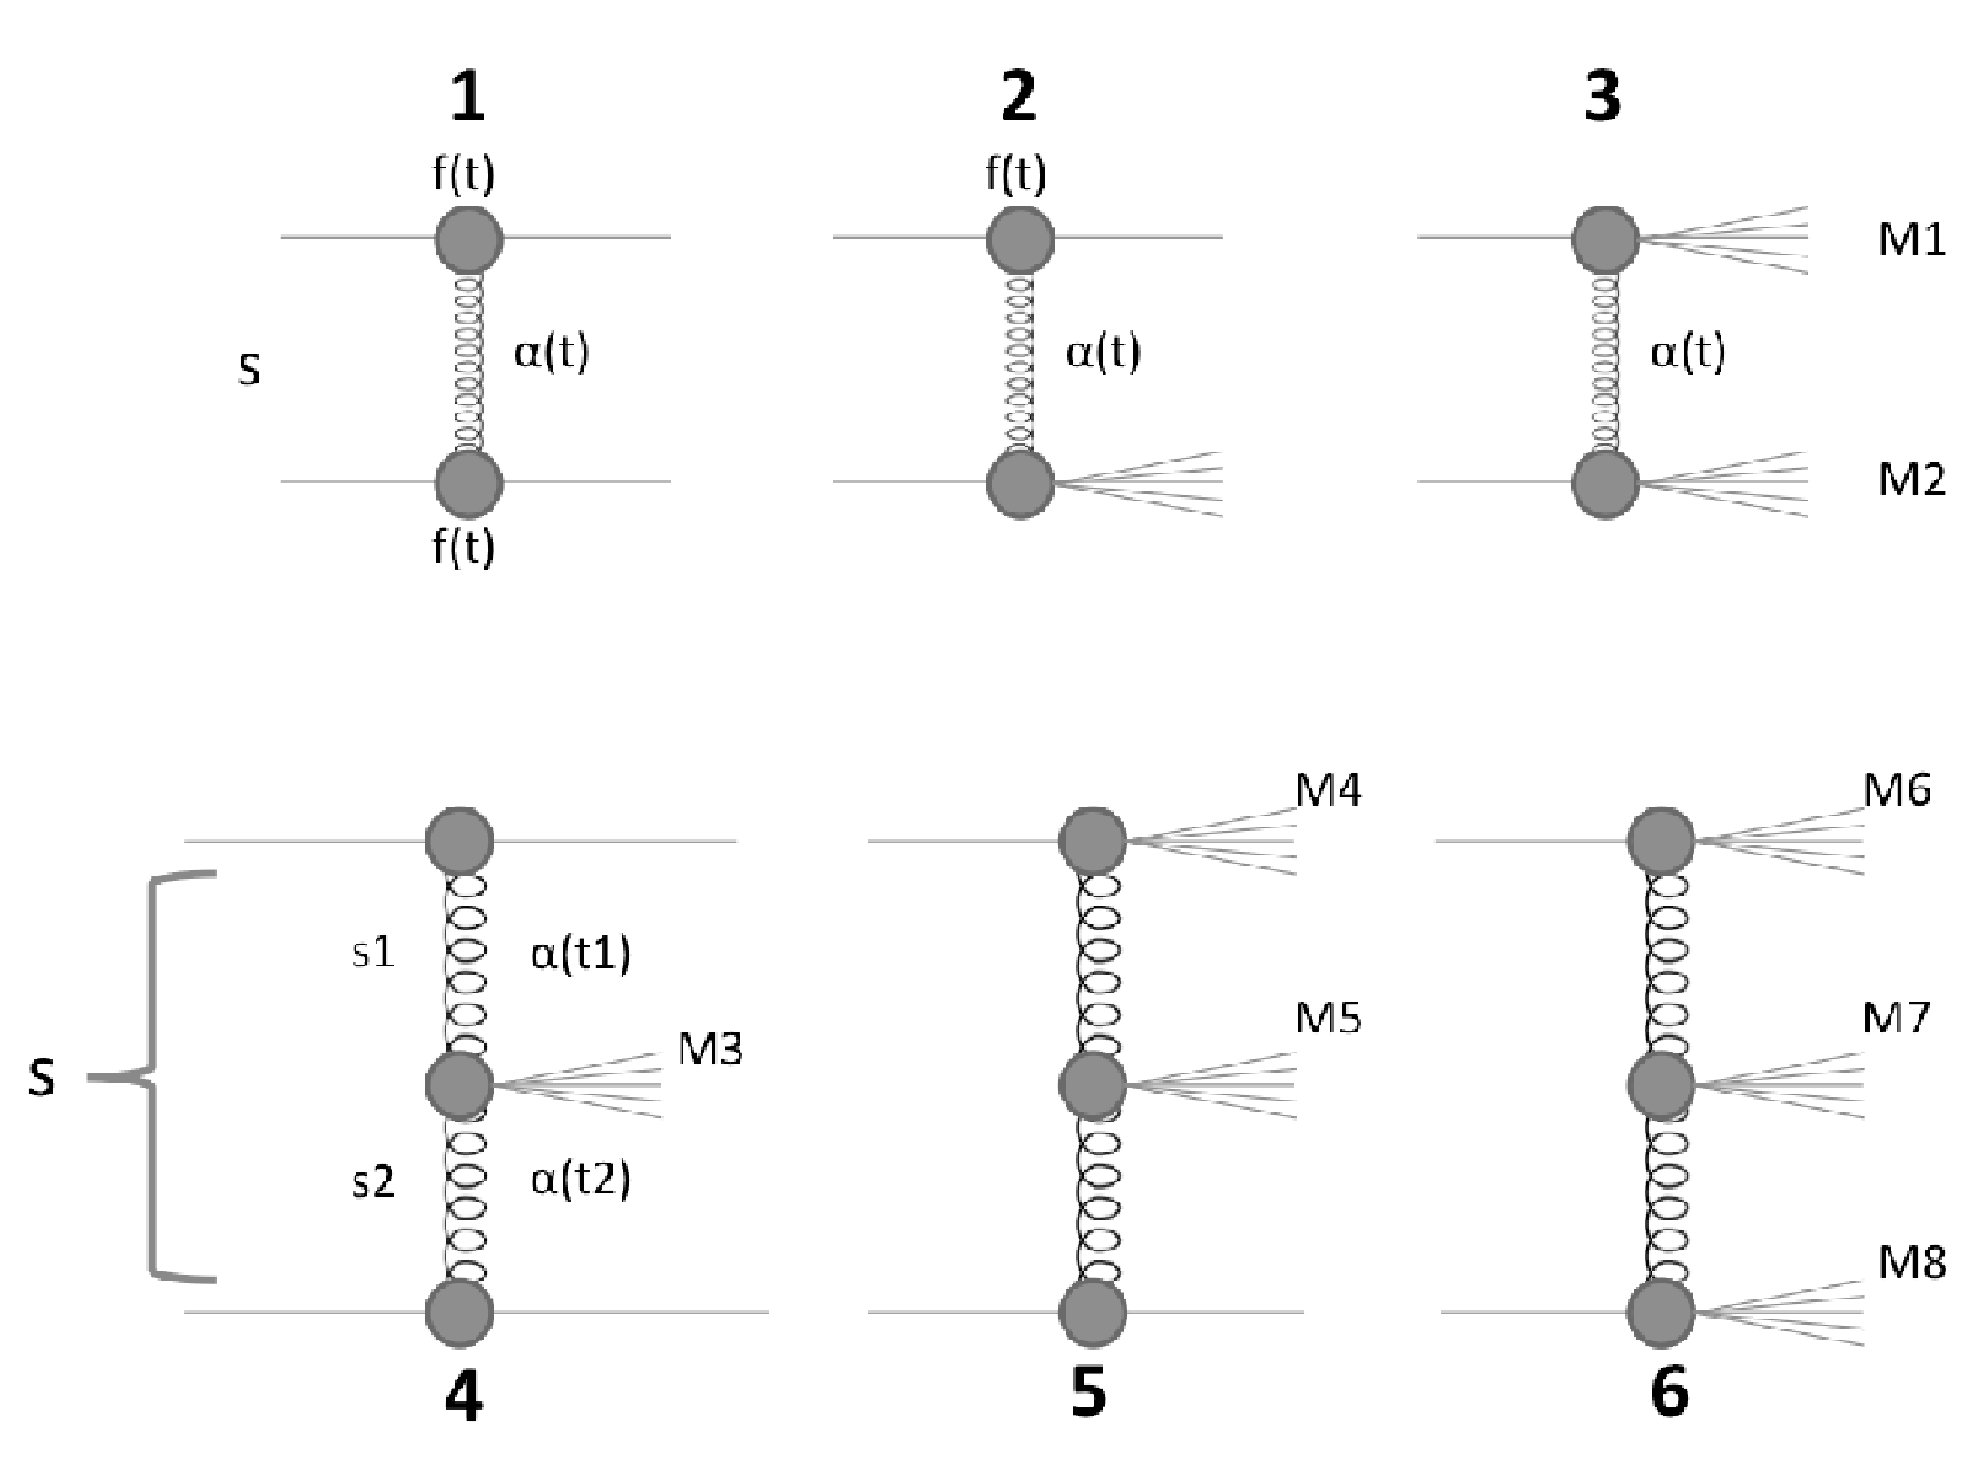
\includegraphics[width=0.5\linewidth]{Fig1.eps}
\caption{Diagrams for elastic scattering and diffraction dissociation (single, double and central).} \label{fig:FeynmanDiagrams}
\end{figure}
% %%%%%%%%%%%%%%%%%%%%%%%%%%%%%%%%%
%%%%%%%%%%%%% 2 %%%%%%%%%%%%%%%%%
\begin{figure}[p] %[!hb]
%\center{
%  \left{}
\includegraphics[width=0.45\linewidth]{Fig2a_xGoul.eps}%
~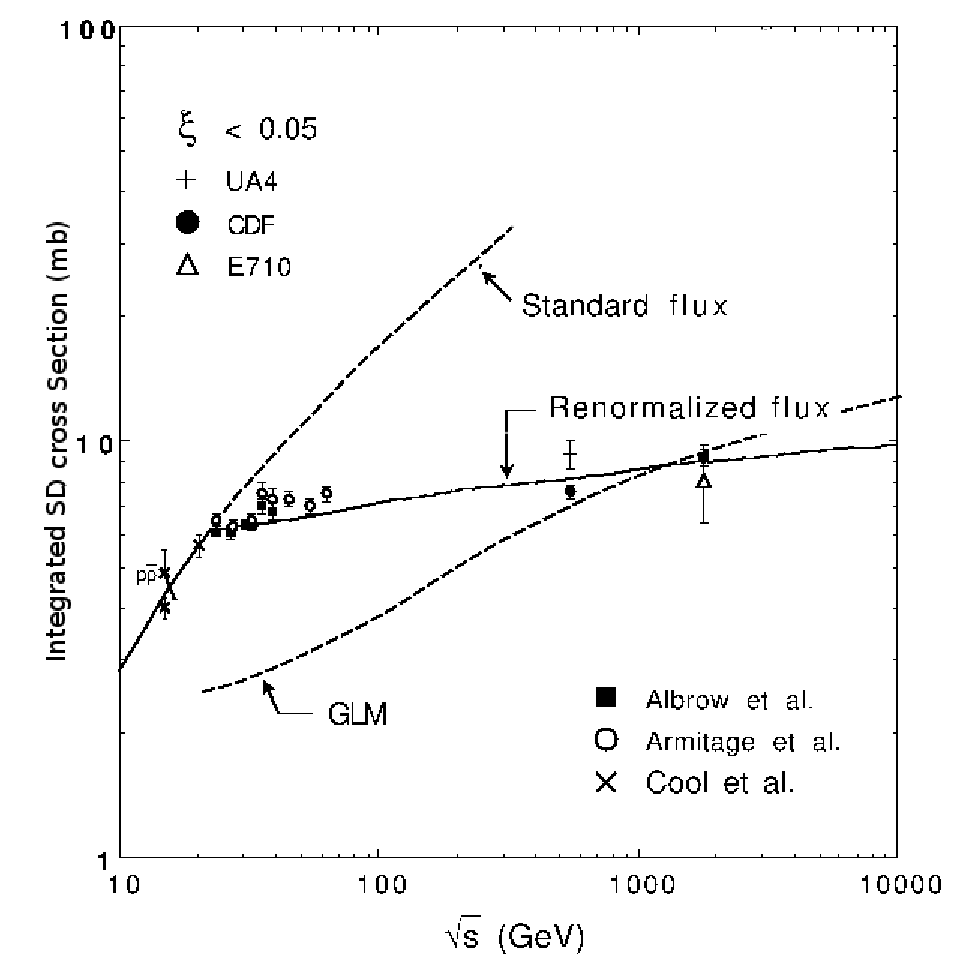
\includegraphics[width=0.4\columnwidth]{Fig2b_cs_goul.eps} \\
  {\hspace{1.5cm} (a)\hspace{0.4\linewidth}(b)}
  \vspace{-0.5cm}
   \caption{(a) Compilation of low-mass SD data from the fixed target $p+d\rightarrow X+d$ Fermilab experiment, at $P_{lab}=275 \mbox{\,GeV/c}$ \cite{Goulianos}. The first peak has the mean value of $M_{X,1}=1400 \mbox{\,MeV}$ and the second bump has $M_{X,2}=1688 \mbox{\,MeV}$, which seems to correspond to the masses of Roper, and $N^*(1680)$ resonances,  see~Sec.~4.2. %\vspace{1cm}
   (b) The integrated single diffraction cross section, renormalized by Goulianos \cite{GoulPlots}.}
   \label{fig1}
  \vspace{-0.5cm} 
\end{figure}
%%%%%%%%%%%%%%%%%%%%%%%%%%%%%%%%%
\newpage
%%%%%%%%%%%%% 3 %%%%%%%%%%%%%%%%%
\begin{figure}[p] %[!bt]
 %\crentering 
 \hspace{1cm} 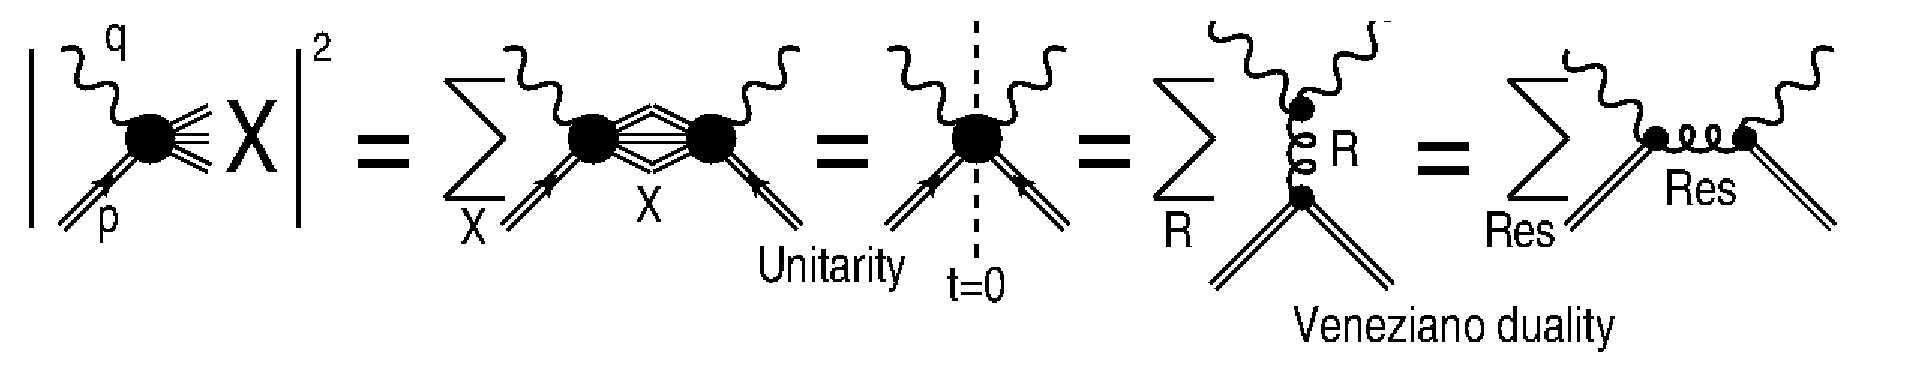
\includegraphics[width=.9\textwidth]{Fig3_diag.eps}
 \caption{Connection, through unitarity (generalized optical
 theorem) and Veneziano-duality, between the inelastic form factor
 and sum of direct-channel resonances.} \label{fig:Regge-dual}
\end{figure}
%%%%%%%%%%%%%%%%%%%%%%%%%%%%%%%%%
%%%%%%%%%%%%% 4 %%%%%%%%%%%%%%%%%
\begin{figure}[p] %[!t]
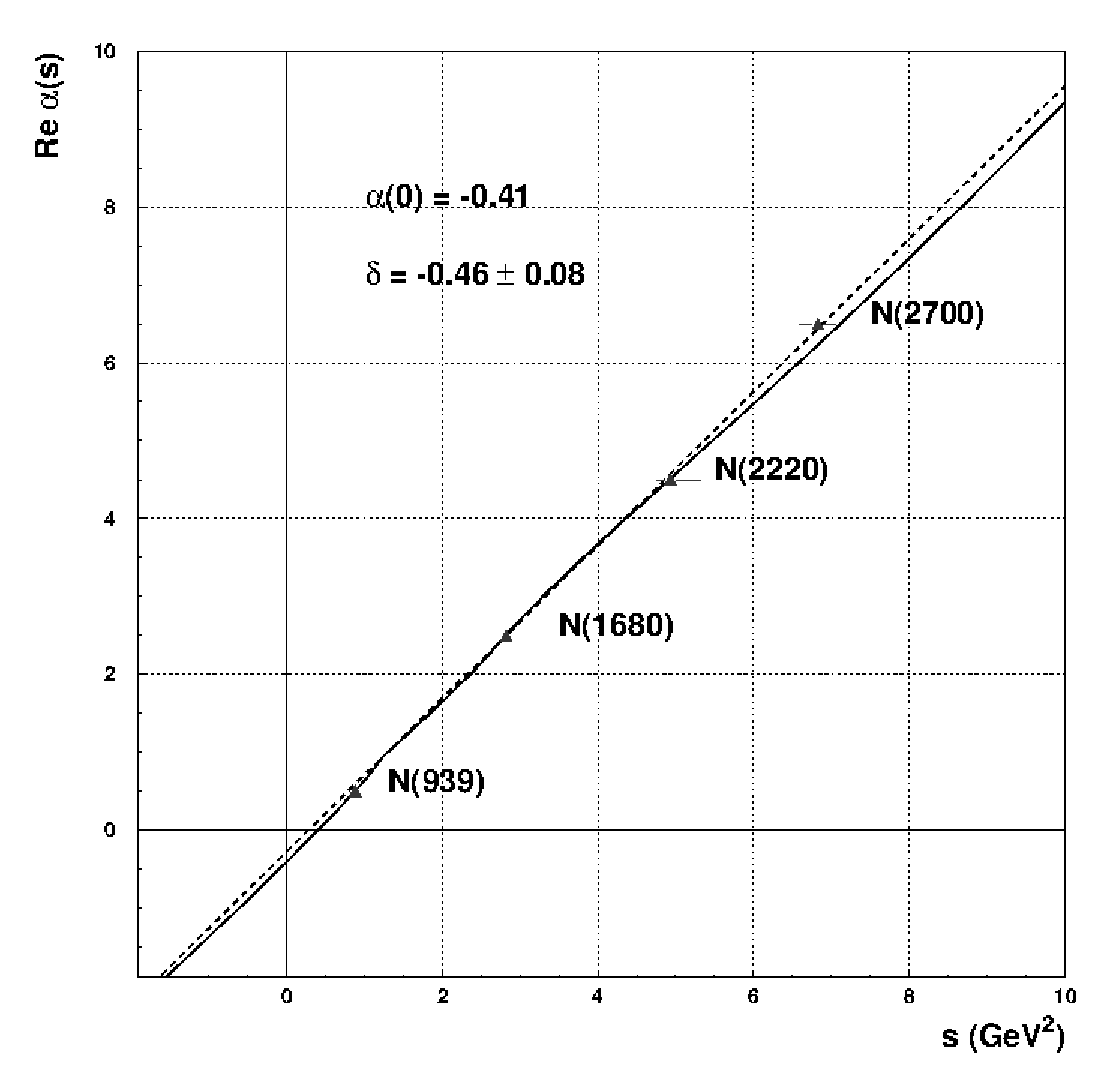
\includegraphics[width=.48\textwidth]{Fig4a_n1.eps}%
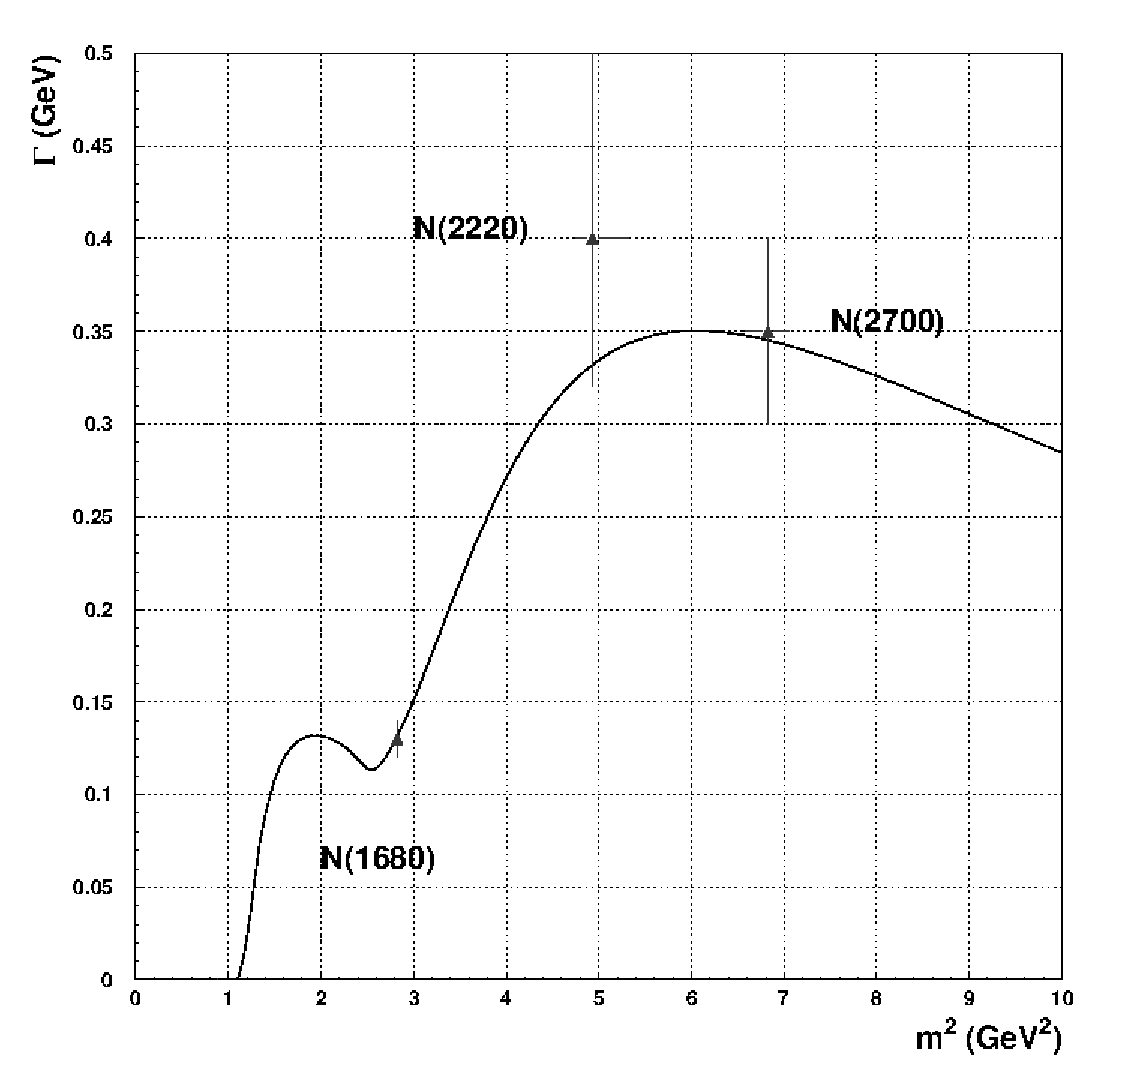
\includegraphics[width=.48\textwidth]{Fig4b_n1width.eps}
\caption{The real (right) and imaginary (left) parts of the proton Regge trajectory. The dashed line corresponds to the result of a linear fit, the solid line is the
fit from \cite{Paccanoni}. \label{fig:n1}}
\end{figure}
%%%%%%%%%%%%%%%%%%%%%%%%%%%%%%%%%
\newpage
%%%%%%%%%% 5(cs(s), dcs/dt SD,Data) %%%%% 
\begin{figure}[p]
  \centering
  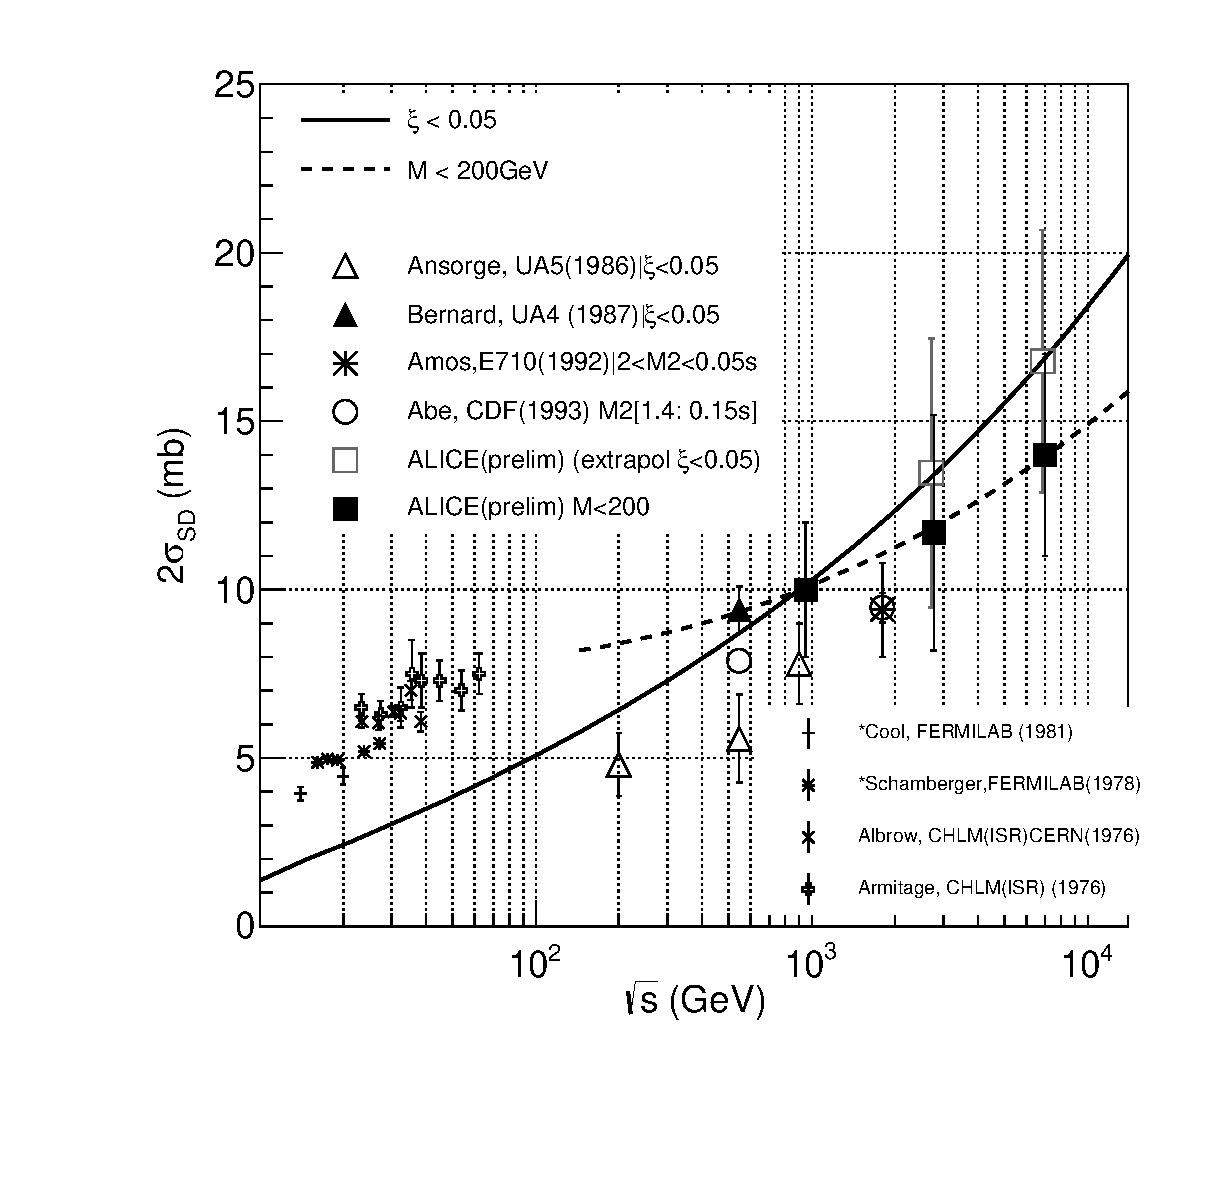
\includegraphics[width=0.49\linewidth,bb=13mm 24mm 195mm 185mm,clip]{Fig5a_cs_sSD.eps}
  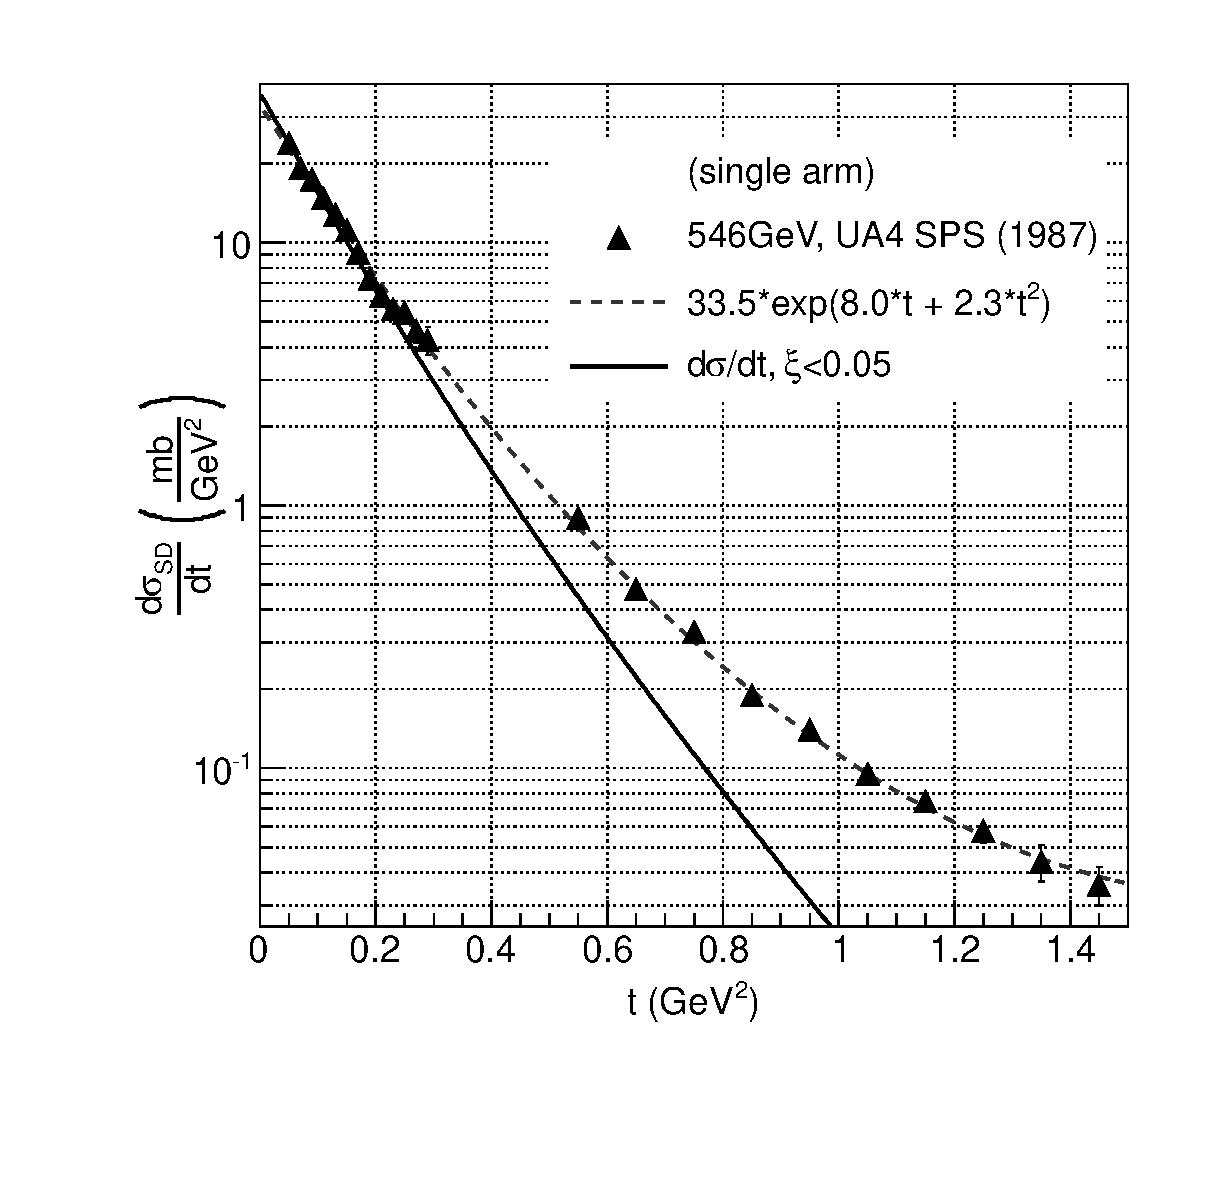
\includegraphics[width=0.49\linewidth,bb=13mm 24mm 195mm 185mm,clip]{Fig5b_dcs_tSD.eps}
  {(a)\hspace{0.5\linewidth}(b)}
  \caption{(a) Single diffraction dissociation cross section vs. energy $\sqrt{s}$ calculated from Eq.~(\ref{SD}). The data are from \cite{Poghosyan for ALICE, [tmp6].Ansorge.UA5, Bernard.UA4.1987, Amos.E710.1992, Abe.CDF.1993} (high energy data), and \cite{lowSD.Cool, lowSD.Schamberger, lowSD.Albrow, lowSD.Armitage} (low energy data). For $\sigma|_{\xi<0.05}$: $\chi^2/$n$=1.6$, n$=6$ (only $\sqrt{s}>100$~GeV) and for $\sigma|_{M<200\mbox{~GeV}}$: $\chi^2/$n$<0.01$, n$=3$. \hspace{4mm}  
  (b) Single differential cross section $\frac{d\sigma_\mathrm{SD}}{dt}$ for SD (single arm) calculated from Eq.~(\ref{SD}), integrated over the region $M_x^2<0.05s$, see \cite{Bernard.UA4.1987}.}
 \label{fig:cs|dcsdt.SD.Data}
\end{figure}
%%%%%%%%%%%%%%%%%%%%%%%%%%%%%%%%%%%%%%%%% 
%%%%%% 6(d2cs/dtdM2, SD, Data) %%%%%%%%%% 
\begin{figure}[p] %[!ht]
  \centering
  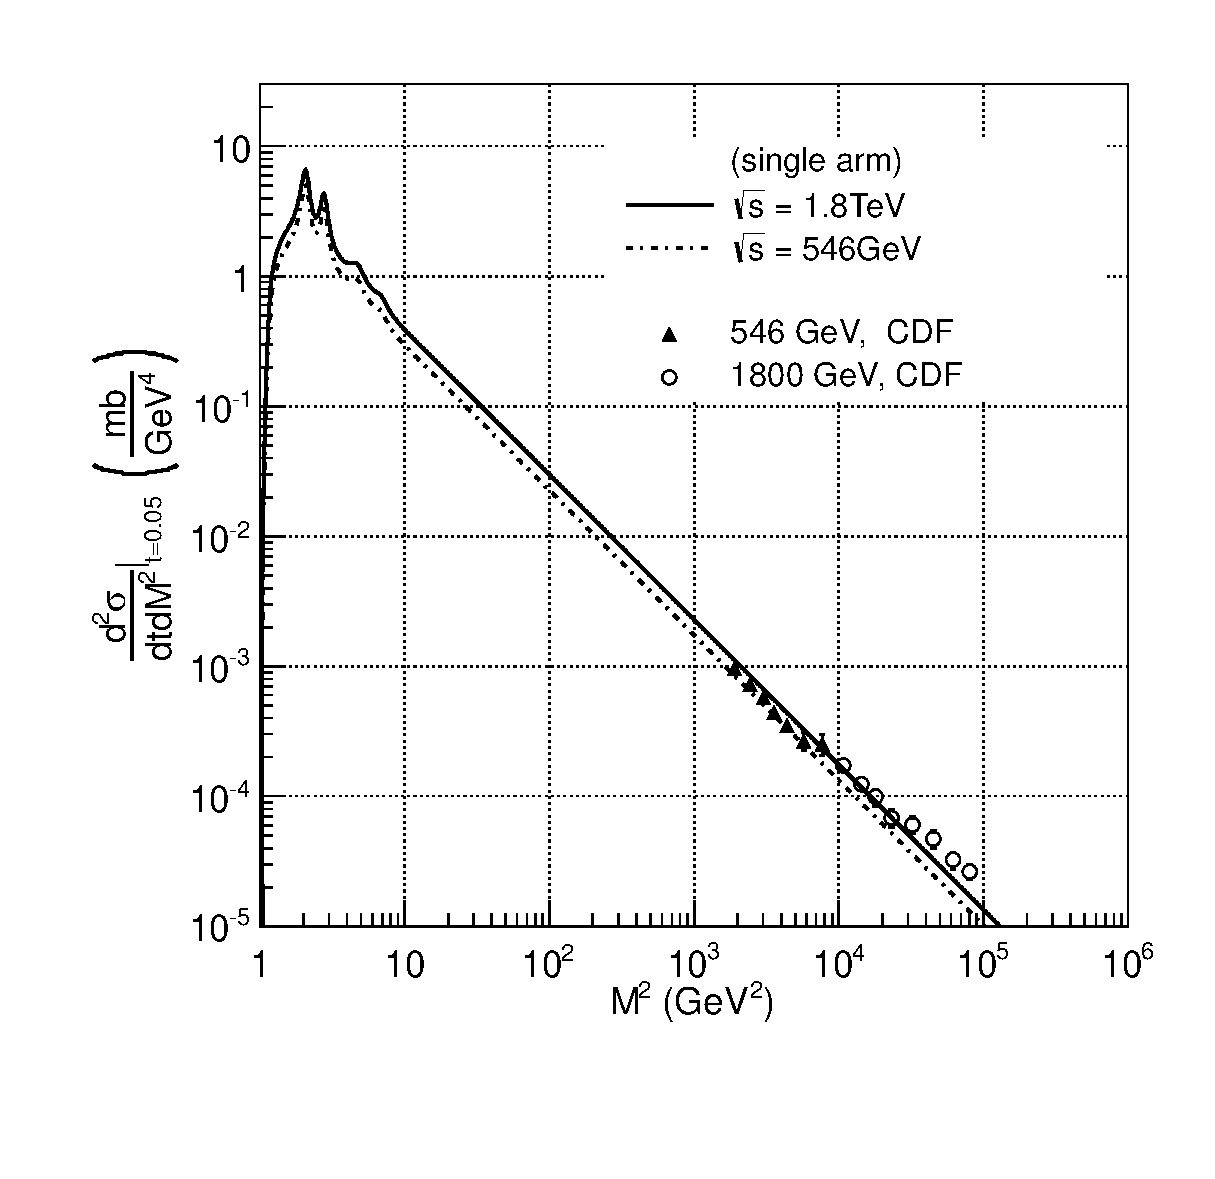
\includegraphics[width=0.49\linewidth,bb=13mm 24mm 195mm 185mm,clip]{Fig6a_gl_t.eps}
  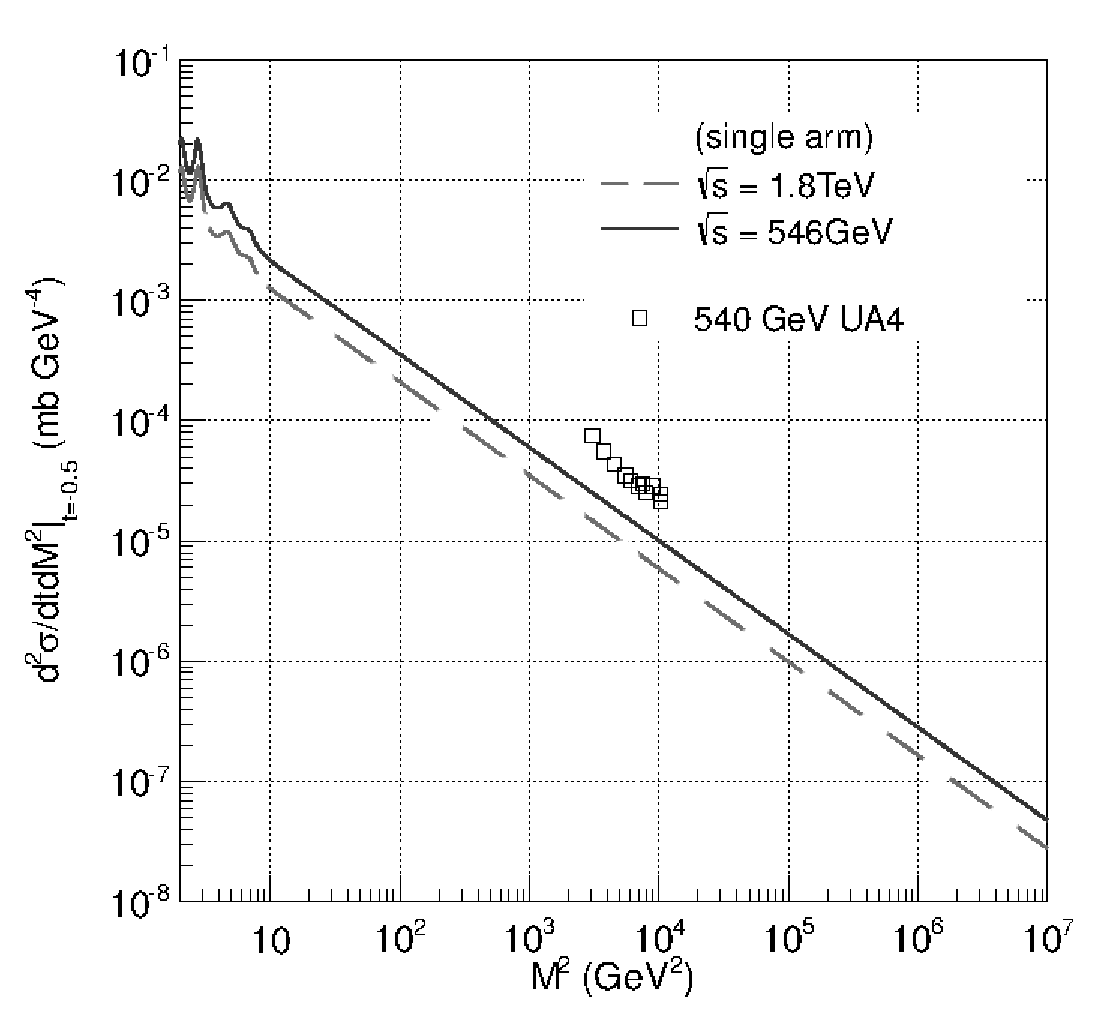
\includegraphics[width=0.49\linewidth]{Fig6b_cl_t.eps}
   {(a)\hspace{0.47\linewidth}(b)}
  \caption{Double differential cross sections for SD (single arm) (a) at $t=-0.05$ (see \cite{Abe.CDF.1993, GoulianosMomtanha}) and (b) at $t=-0.5$ (see \cite{Bozzo.SD_t0.55}) with theoretical predictions calculated from Eq.~(\ref{SD}); $\chi^2/$n$=1.2$, n$=8$ for $1800$~GeV$^2$ and $\chi^2/$n$=4.6$, n$=8$ for $546$~GeV$^2$  (only Fig.~(a));}
 \label{fig:d2cs.SD.Data}
\end{figure}
%%%%%%%%%%%%%%%%%%%%%%%%%%%%%%%%%%%%%%%%% 
\newpage
%%%%%%%% 7(d2cs/dtdM2, SD) %%%%%%%%%%%%%% 
\begin{figure}[p] %[!ht]
 \centering
 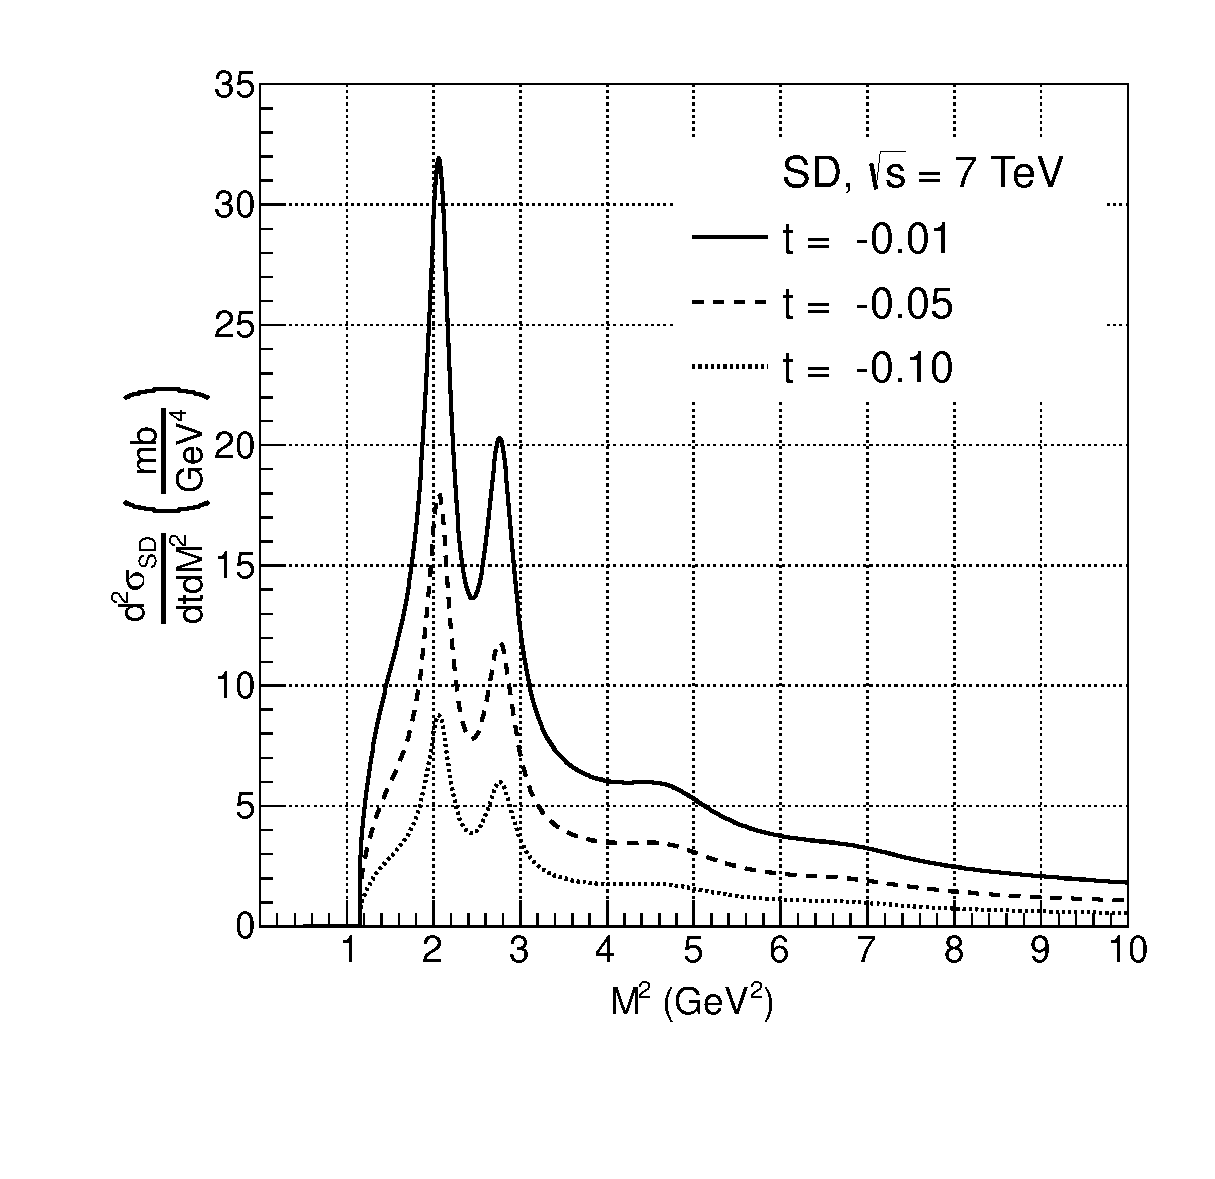
\includegraphics[width=0.49\linewidth,bb=13mm 24mm 195mm 185mm,clip]{Fig7a_d2cs_m2.eps}
 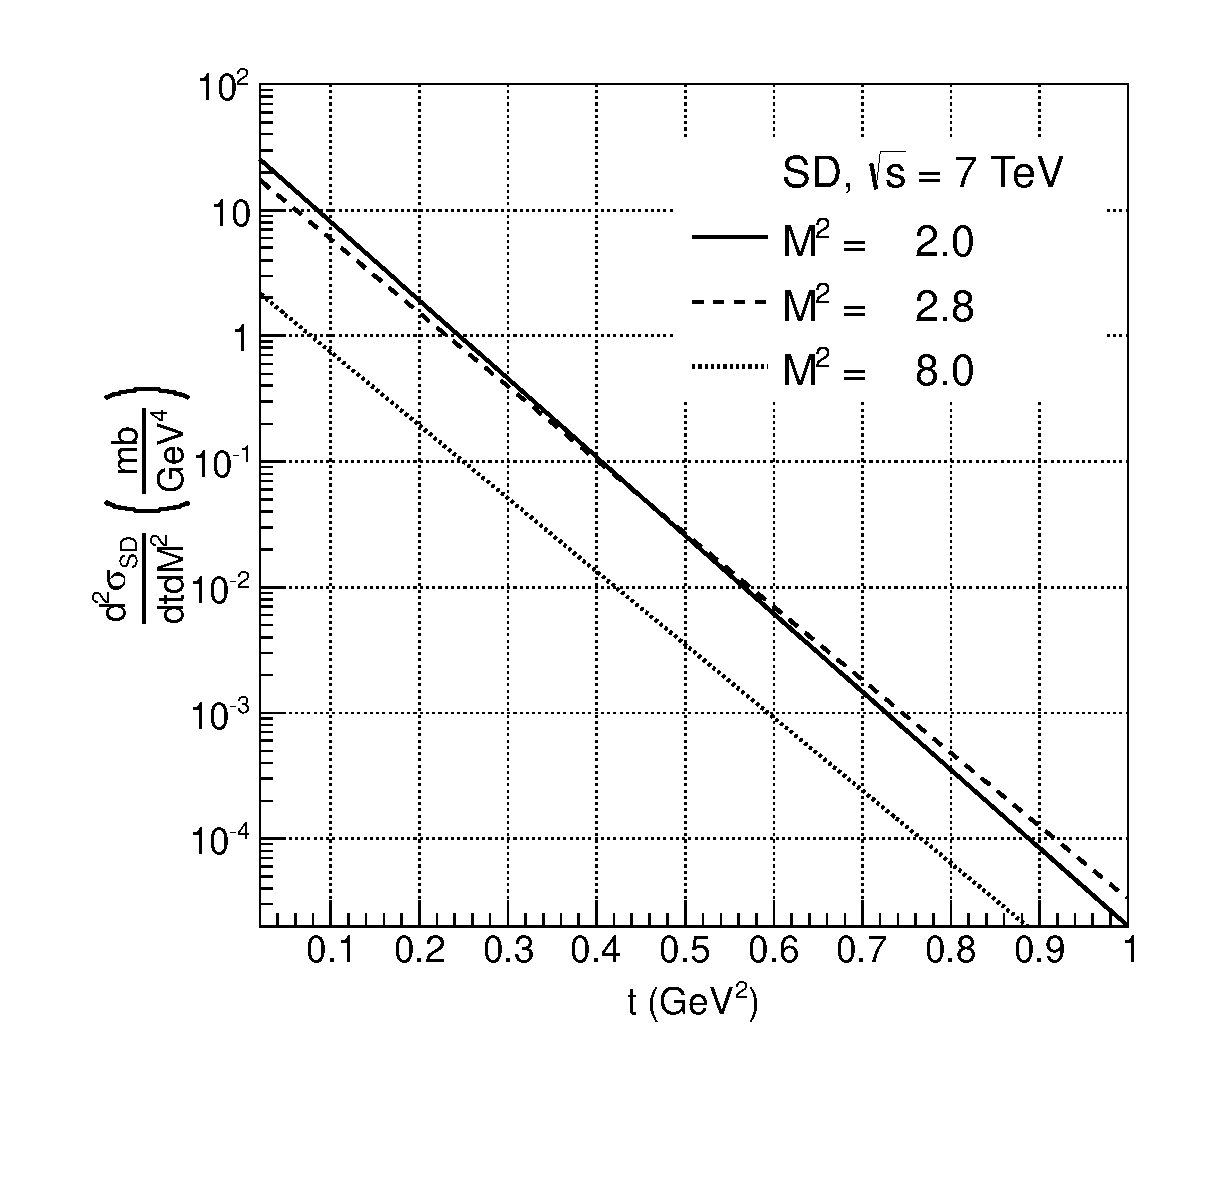
\includegraphics[width=0.49\linewidth,bb=13mm 24mm 195mm 185mm,clip]{Fig7b_d2cs_t.eps}
  {(a)\hspace{0.47\linewidth}(b)}
 \caption{Double differential SD cross sections (single arm) (a) as functions of $M^2$ for different $t$ values, and (b) as functions of $t$ for different $M^2$ values, see Eq.~(\ref{SD}).}
 \label{d2cs_m2.in.t}
\end{figure}
%%%%%%%%%%%%%%%%%%%%%%%%%%%%%%%%%%%%%%%%% 
%%%%%%%%% 8(cs, DD, Data) %%%%%%%%%%%%%%% 
\begin{figure}[p] %[!ht]
 {\centering
 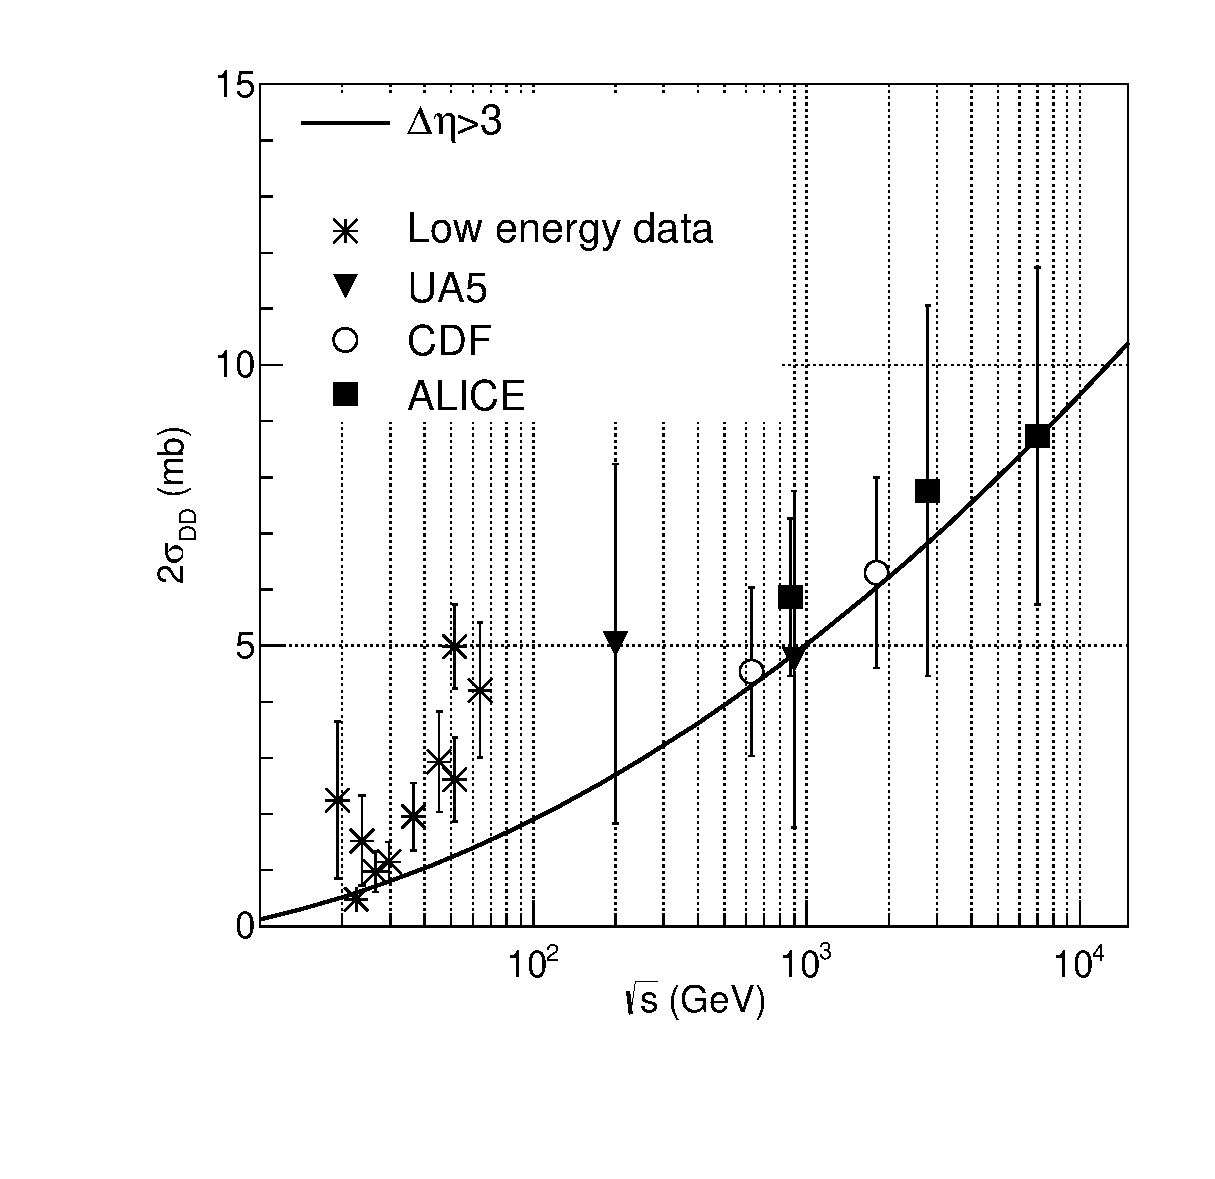
\includegraphics[width=0.47\linewidth,bb=13mm 24mm 195mm 185mm,clip]{Fig8a_cs_sDD.eps}
 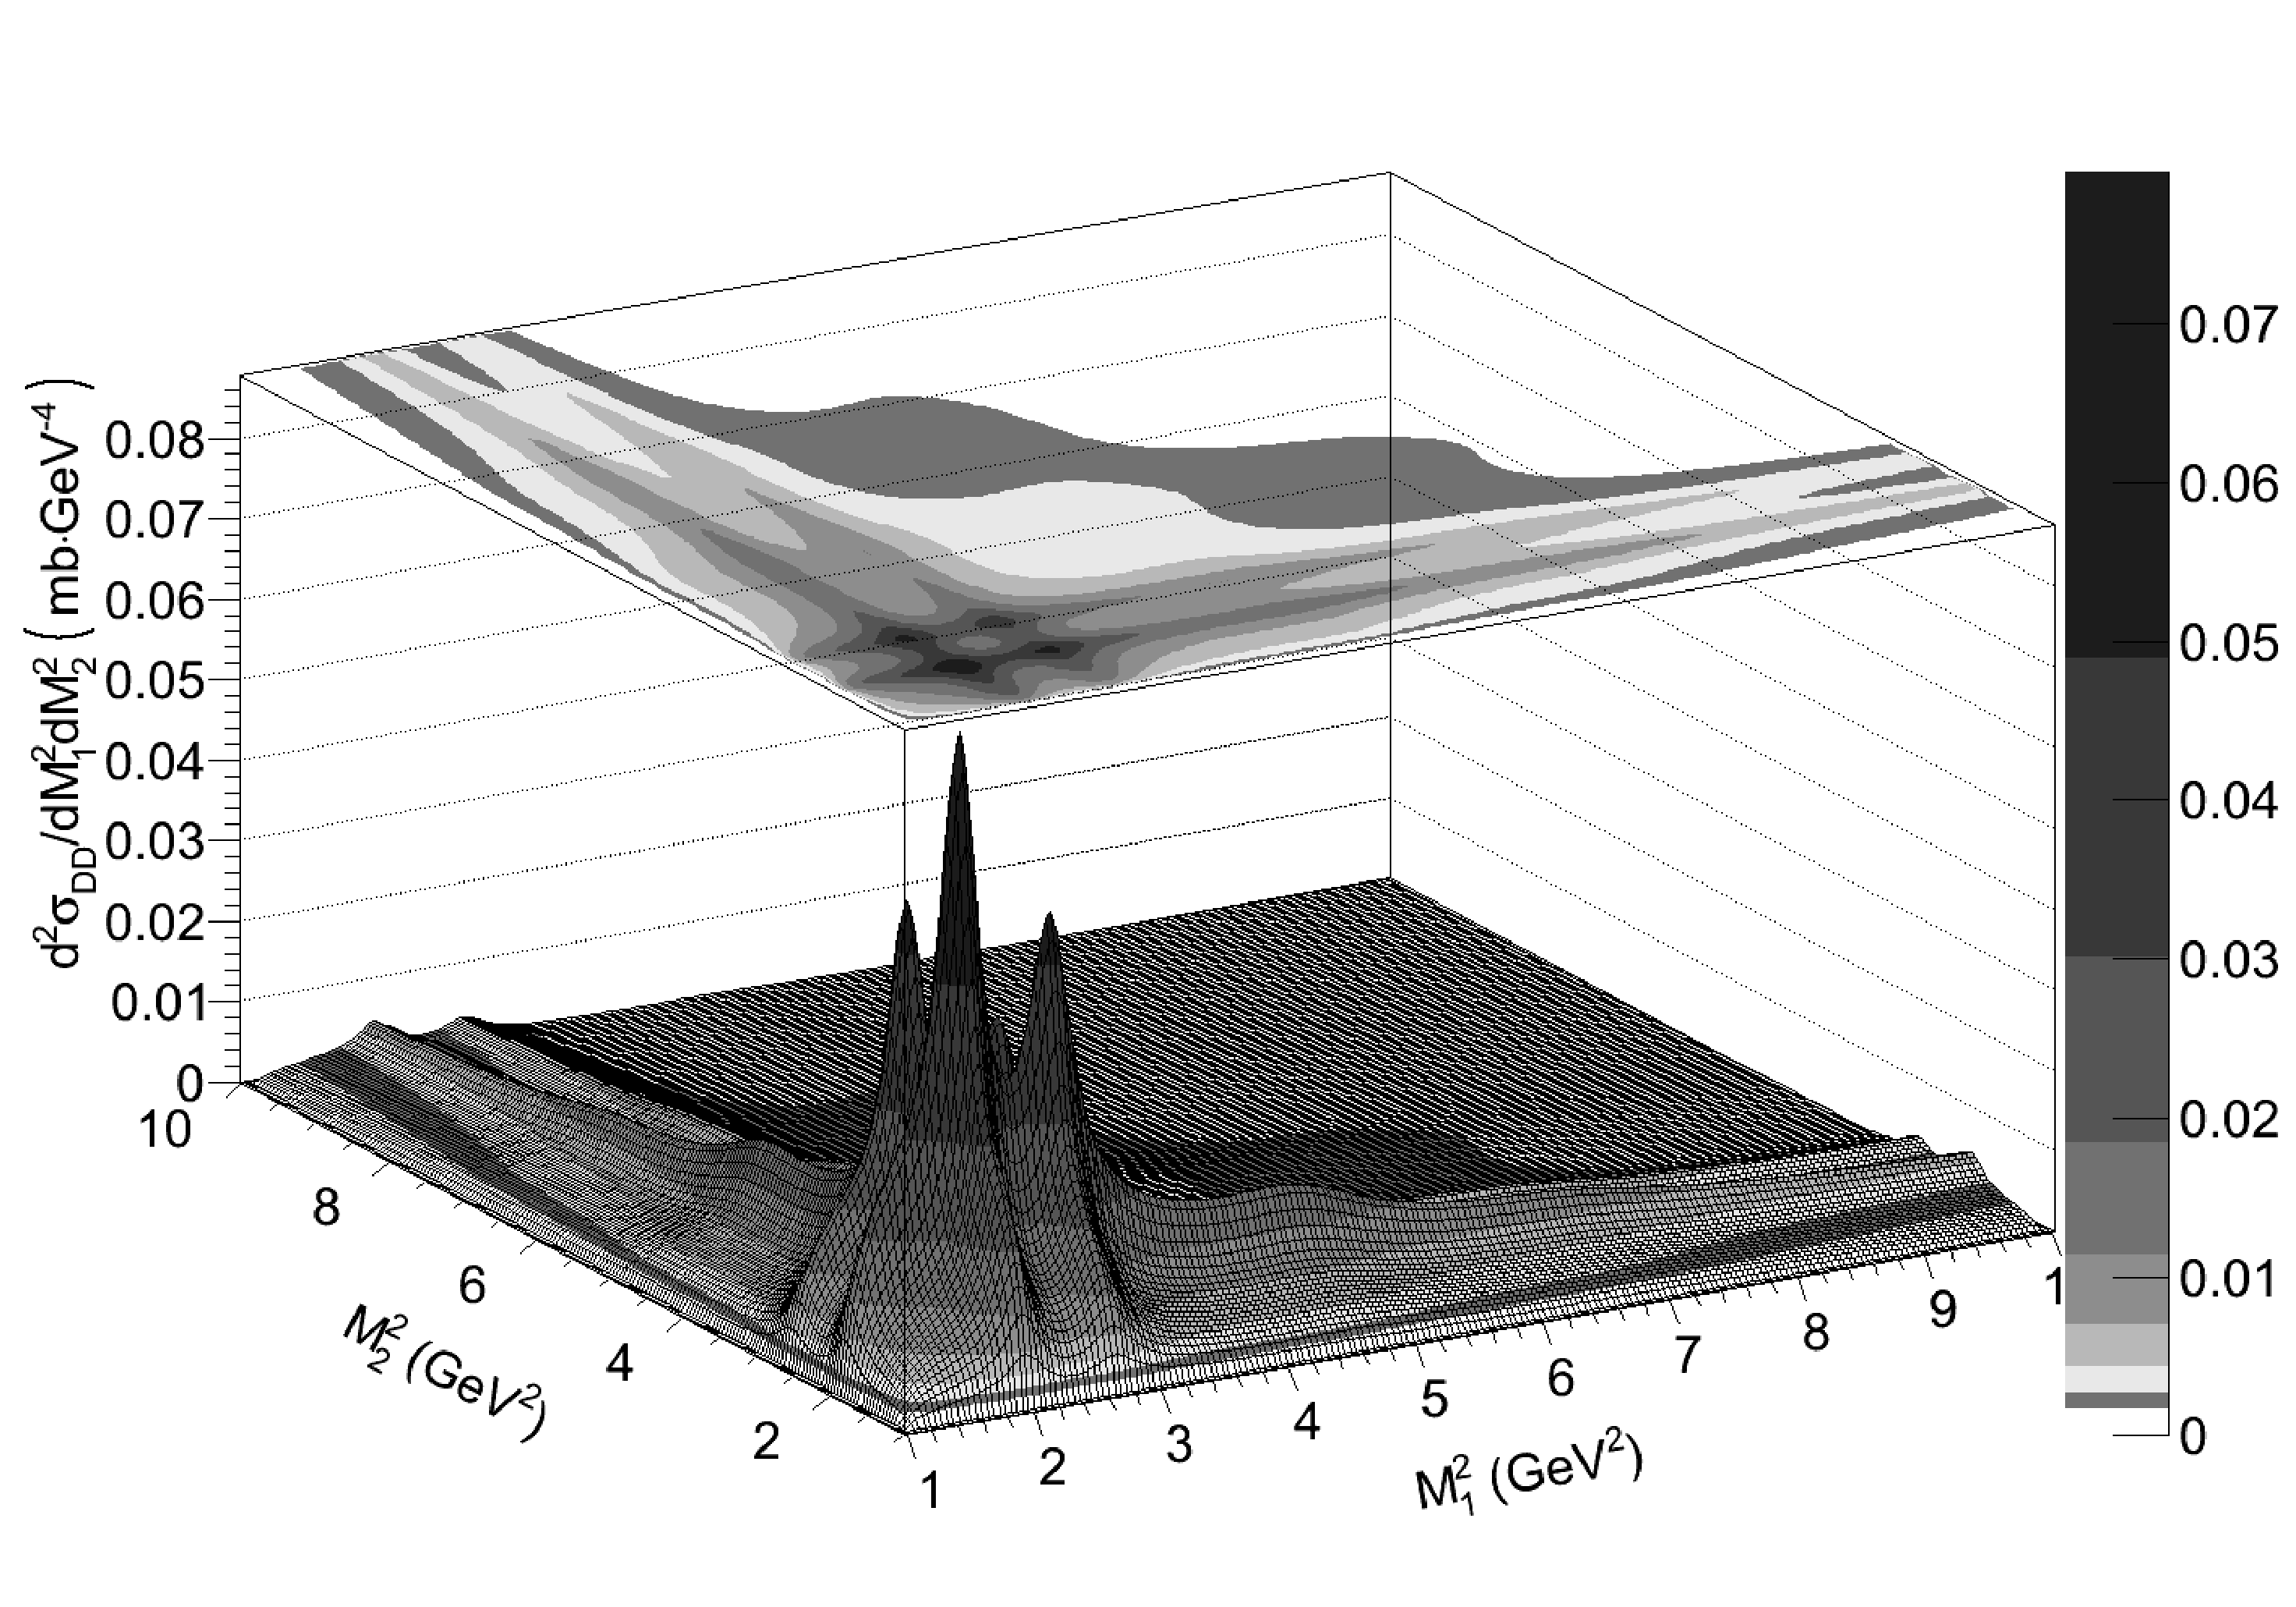
\includegraphics[width=0.5\linewidth,bb=0 0 1400 900,clip]{Fig8b_int_t_DD_2D.eps}
 {(a)\hspace{0.5\linewidth}(b)}
 }
  \caption{
  (a) The double diffraction dissociation cross section vs. energy $\sqrt{s}$ calculated from Eq.~(\ref{DD}).
  Experimental data are from \cite{Poghosyan for ALICE, Affolder.DD, [tmp6].Ansorge.UA5}; $\chi^2/$n$=0.2$, n$=7$, for $\sqrt{s}>100$~GeV only. Note that here we account for two configurations of dissociated systems, namely $(M_{x_1},M_{x_2})$ and $(M_{x_2},M_{x_1})$, thus here \mbox{$\sigma_\mathrm{DD}=2\sigma^{\mbox{theor}}_\mathrm{DD}$};
    (b) The double differential DD cross section as a function of $M_1^2$ and $M_2^2$ integrated over $t$; see Eq.~(\ref{DD}). Here only half of the cross section is depicted, since only one mode (arm) is considered.}
  \label{cs.DD}
\end{figure}
%@@@@@@@@@@@@@@@@@@@@@@@@@@@@@@@@@@@@@@@@@@@@@@@@@@@@@@@@@@

\newpage
\newpage

%~~~~~~~~~~~~~~~~~~~~~~~~~~~~~~~~~~~~~~~~~~~~~~~~~~~~~~~~~
 \begin{table}[p] %[!ht]
  \centering
  \caption{\label{tab:cs.el} $pp$ elastic cross section [mb]  Eq.~(\ref{elastic}), and forward slope [GeV$^{-2}$] calculated with the parameters quoted in Tab. \ref{tab:ParSet}.}
%    \begin{tabular}{0.97\columnwidth}{|c||c|c||c|c|}
    \begin{tabular}{|c||c|c||c|c|}
      \hline
$\sqrt{s}$[TeV]&$\sigma_\mathrm{el}^{\mathrm{\,th}}$&$\sigma_\mathrm{el}^{\mathrm{\,exp}}$
                                                              &$B_\mathrm{el}^{\mathrm{\,th} }$&$B_\mathrm{el}^{\mathrm{\,exp} }$ \\ \hline
          $7$  &   $24.5$ &$25.4\pm1.1$ \cite{[T1].TOTEM}          &$19.79$&$19.9 \pm0.3$ \cite{[T1].TOTEM}         \\ \hline
          $1.8$&   $17.99$&$16.6\pm1.6$ \cite{[tmp3]Amos.E710.[3]} &$17.94$&$17.0 \pm0.5$ \cite{[tmp3]Amos.E710.[3]}\\
               &          &                                        &       &$17.9 \pm2.5$ \cite{[tmp3]Amos.E710.[5]}\\
               &          &                                        &       &$16.99$       \cite{Abe.CDF.1993}      \\ \hline
        $0.546$&   $13.8$ &$13.6$      \cite{Bozzo1}               &$16.32$&$15.35$       \cite{Abe.CDF.1993}      \\
               &          &                                        &       &$15.0$ \cite{[tmp6].Ansorge.UA5}        \\ \hline
    \end{tabular}
 \end{table}
\begin{table}[p] %[t]
\centering
 \caption{\label{tab:ParSet} Fitted parameters of the model, see Eqs.~(\ref{elastic}), (\ref{SD}), (\ref{DD}).}
  \begin{tabular}{cc}
%     \begin{tabular*}{0.4\columnwidth}{|c||c|}
     \begin{tabular}{|c||c|}
        \hline
        $A_\mathrm{el}[$mb$]$         & $33.58$\\
        $b_\mathrm{el}[$GeV$^{-2}]$ &$1.937$\\ \hline

    $A_\mathrm{res}[$mb$\cdot$GeV$^4]$&$2.21$\\
        $C_\mathrm{bg}[$mb$]$         &$2.07$\\
        $R$                  &$0.45$\\
        $b_\mathrm{res}[$GeV$^{-2}]$&$-0.507$\\
        $b_\mathrm{bg}[$GeV$^{-2}]$ &$-1.013$\\ \hline
     \end{tabular}&
%     \begin{tabular}{0.34\columnwidth}{|c||c|}
     \begin{tabular}{|c||c|}
        \hline
        \multicolumn{2}{|c|}{$\alpha(t)=\alpha(0)+\alpha't$}\\ \hline
        $\alpha(0)$           & $1.075$\\
        $\alpha'$[GeV$^{-2}$] & $0.34$\\\hline
        \hline
        $s_0$      &$1$\\ \hline
        $\varsigma$&$0.8$\\
        $\eta$     &$1$\\ \hline
     \end{tabular}%
  \end{tabular}%
\end{table}
%################################
\begin{table}[p] %[!t]
  \centering
  \caption{\label{tab:cs.predict}Predictions (in [mb]) for SD and DD at 7, 8 and 13~TeV.}
%  \begin{tabular*}{0.85\columnwidth}{|c||c|c||r|}
  \begin{tabular}{|c||c|c||r|}
       \hline
       $\sqrt{s} [$~TeV$]$& $\sigma_\mathrm{SD}|_{M<200GeV}$& $\sigma_\mathrm{SD}|_{\xi<0.05}$
                                         & $\sigma_\mathrm{DD}|_{\Delta\eta>3}$\\  \hline
        7&13.96& 16.87& 8.63 \\
        8&14.30& 17.43& 8.93 \\
       13&15.67& 19.59&10.09 \\ \hline
   \end{tabular}
\end{table}
%################################
\begin{table}[p] %[t]
  \centering
  \caption{\label{tab:cs.SD.DD.res} Cross sections [mb] calculated below the upper integrational limit, shown in the table.}
  \begin{tabular}{c|c}
%     \begin{tabular*}{0.925\columnwidth}{|l||c|c||c|c||c|c|}
     \begin{tabular}{|c||c|c||c|c||c|c}
       \hline
       $\sqrt{s}$&\multicolumn{2}{c||}{$M_x<\eta_\mathrm{SD}$ [GeV]}&\multicolumn{4}{c}{$M_{x_1}+M_{x_2}<\eta_\mathrm{DD}$ [GeV]}\\ \cline{2-7}
 $[$TeV$]$&$\sigma_\mathrm{SD}$&$\eta_\mathrm{SD}$&
            $\sigma_\mathrm{DD}$&$\eta_\mathrm{DD}$&
            $\sigma_\mathrm{DD}$&$\eta_\mathrm{DD}$       \\ \hline
        7& 5.05&3.4& 0.93&6.8& 0.20&3.4\\
        8& 5.37&3.6& 1.01&7.2& 0.26&3.6\\
       13& 6.29&4.0& 1.21&8.0& 0.40&4.0\\ \hline
     \end{tabular}%
  \end{tabular}%
\end{table}

\end{document}
